% !TeX encoding = UTF-8
% !TeX program = xelatex
% !TeX spellcheck = en_US

\documentclass[degree=bachelor, fontset=windows]{thuthesis}
  % 学位 degree:
  %   doctor | master | bachelor | postdoc
  % 学位类型 degree-type:
  %   academic(默认)| professional
  % 语言 language
  %   chinese(默认)| english
  % 字体库 fontset
  %   windows | mac | fandol | ubuntu
  % 建议终版使用 Windows 平台的字体编译


% 论文基本配置,加载宏包等全局配置
% !TeX root = ./thuthesis-example.tex

% 论文基本信息配置

\thusetup{
  %******************************
  % 注意:
  %   1. 配置里面不要出现空行
  %   2. 不需要的配置信息可以删除
  %   3. 建议先阅读文档中所有关于选项的说明
  %******************************
  %
  % 输出格式
  %   选择打印版(print)或用于提交的电子版(electronic),前者会插入空白页以便直接双面打印
  %
  output = print,
  % 格式类型
  %   默认为论文(thesis),也可以设置为开题报告(proposal)
  % thesis-type = proposal,
  %
  % 标题
  %   可使用“\\”命令手动控制换行
  %
  title  = {卢非酰胺连续合成过程可调鲁棒优化设计方法研究},
  title* = {Adjustable Robust Optimization for the Process Design of Continuous Rufinamide synthesis},
  %
  % 学科门类
  %   1. 学术型
  %      - 中文
  %        需注明所属的学科门类,例如:
  %        哲学、经济学、法学、教育学、文学、历史学、理学、工学、农学、医学、
  %        军事学、管理学、艺术学
  %      - 英文
  %        博士:Doctor of Philosophy
  %        硕士:
  %          哲学、文学、历史学、法学、教育学、艺术学门类,公共管理学科
  %          填写“Master of Arts“,其它填写“Master of Science”
  %   2. 专业型
  %      直接填写专业学位的名称,例如:
  %      教育博士、工程硕士等
  %      Doctor of Education, Master of Engineering
  %   3. 本科生不需要填写
  %
  %degree-category  = {工学硕士},
  %degree-category* = {Master of Science},
  %
  % 培养单位
  %   填写所属院系的全名
  %
  department = {探微书院},
  %
  % 学科
  %   1. 研究生学术型学位,获得一级学科授权的学科填写一级学科名称,其他填写二级学科名称
  %   2. 本科生填写专业名称,第二学位论文需标注“(第二学位)”
  %
  discipline  = {化学生物学+化学工程与工业生物工程},
  discipline* = {},
  %
  % 专业领域
  %   1. 设置专业领域的专业学位类别,填写相应专业领域名称
  %   2. 2019 级及之前工程硕士学位论文,在 `engineering-field` 填写相应工程领域名称
  %   3. 其他专业学位类别的学位论文无需此信息
  %
  % professional-field  = {计算机技术},
  % professional-field* = {Computer Technology},
  %
  % 姓名
  %
  author  = {邱韬宇},
  author* = {Qiu Taoyu},
  %
  % 学号
  % 仅当书写开题报告时需要(同时设置 `thesis-type = proposal')
  %
  % student-id = {2000310000},
  %
  % 指导教师
  %   中文姓名和职称之间以英文逗号“,”分开,下同
  %
  supervisor  = {袁志宏, 副教授},
  supervisor* = {Assoc. Professor Yuan Zhihong},
  %
  % 副指导教师
  %
  %associate-supervisor  = {陈文光, 教授},
  %associate-supervisor* = {Professor Chen Wenguang},
  %
  % 联合指导教师
  %
  % co-supervisor  = {某某某, 教授},
  % co-supervisor* = {Professor Mou Moumou},
  %
  % 日期
  %   使用 ISO 格式;默认为当前时间
  %
  % date = {2019-07-07},
  %
  % 是否在中文封面后的空白页生成书脊(默认 false)
  %
  include-spine = false,
  %
  % 密级和年限
  %   秘密, 机密, 绝密
  %
  % secret-level = {秘密},
  % secret-year  = {10},
  %
  % 博士后专有部分
  %
  % clc                = {分类号},
  % udc                = {UDC},
  % id                 = {编号},
  % discipline-level-1 = {计算机科学与技术},  % 流动站(一级学科)名称
  % discipline-level-2 = {系统结构},          % 专业(二级学科)名称
  % start-date         = {2011-07-01},        % 研究工作起始时间
}

% 载入所需的宏包

% 定理类环境宏包
\usepackage{amsthm}
% 也可以使用 ntheorem
% \usepackage[amsmath,thmmarks,hyperref]{ntheorem}

\thusetup{
  %
  % 数学字体
  % math-style = GB,  % GB | ISO | TeX
  math-font  = xits,  % stix | xits | libertinus
}

% 可以使用 nomencl 生成符号和缩略语说明
% \usepackage{nomencl}
% \makenomenclature

% 表格加脚注
\usepackage{threeparttable}

% 表格中支持跨行
\usepackage{multirow}

% 固定宽度的表格。
% \usepackage{tabularx}

% 跨页表格
\usepackage{longtable}

% 算法
\usepackage{algorithm}
\usepackage{algorithmic}

% 量和单位
\usepackage{siunitx}

% 参考文献使用 BibTeX + natbib 宏包
% 顺序编码制
\usepackage[sort]{natbib}
%\bibliographystyle{thuthesis-numeric}

% 著者-出版年制
% \usepackage{natbib}
% \bibliographystyle{thuthesis-author-year}

% 生命科学学院要求使用 Cell 参考文献格式(2023 年以前使用 author-date 格式)
% \usepackage{natbib}
% \bibliographystyle{cell}

% 本科生参考文献的著录格式
% \usepackage[sort]{natbib}
\bibliographystyle{thuthesis-bachelor}

% 参考文献使用 BibLaTeX 宏包
% \usepackage[style=thuthesis-numeric]{biblatex}
% \usepackage[style=thuthesis-author-year]{biblatex}
% \usepackage[style=gb7714-2015]{biblatex}
% \usepackage[style=apa]{biblatex}
% \usepackage[style=mla-new]{biblatex}
% 声明 BibLaTeX 的数据库
% \addbibresource{ref/refs.bib}

% 定义所有的图片文件在 figures 子目录下
\graphicspath{{figures/}}

% 数学命令
\makeatletter
\newcommand\dif{%  % 微分符号
  \mathop{}\!%
  \ifthu@math@style@TeX
    d%
  \else
    \mathrm{d}%
  \fi
}
\makeatother

% hyperref 宏包在最后调用
\usepackage{hyperref}



\begin{document}

% 封面
\maketitle

% 学位论文指导小组、公开评阅人和答辩委员会名单
% 本科生不需要
%% !TeX root = ../thuthesis-example.tex

\begin{committee}[name={学位论文指导小组、公开评阅人和答辩委员会名单}]

  \newcolumntype{C}[1]{@{}>{\centering\arraybackslash}p{#1}}

  \section*{指导小组名单}

  \begin{center}
    \begin{tabular}{C{3cm}C{3cm}C{9cm}@{}}
      李XX & 教授     & 清华大学 \\
      王XX & 副教授   & 清华大学 \\
      张XX & 助理教授 & 清华大学 \\
    \end{tabular}
  \end{center}


  \section*{公开评阅人名单}

  \begin{center}
    \begin{tabular}{C{3cm}C{3cm}C{9cm}@{}}
      刘XX & 教授   & 清华大学                    \\
      陈XX & 副教授 & XXXX大学                    \\
      杨XX & 研究员 & 中国XXXX科学院XXXXXXX研究所 \\
    \end{tabular}
  \end{center}


  \section*{答辩委员会名单}

  \begin{center}
    \begin{tabular}{C{2.75cm}C{2.98cm}C{4.63cm}C{4.63cm}@{}}
      主席 & 赵XX                  & 教授                    & 清华大学       \\
      委员 & 刘XX                  & 教授                    & 清华大学       \\
          & \multirow{2}{*}{杨XX} & \multirow{2}{*}{研究员} & 中国XXXX科学院 \\
          &                       &                         & XXXXXXX研究所  \\
          & 黄XX                  & 教授                    & XXXX大学       \\
          & 周XX                  & 副教授                  & XXXX大学       \\
      秘书 & 吴XX                  & 助理研究员              & 清华大学       \\
    \end{tabular}
  \end{center}

\end{committee}



% 也可以导入 Word 版转的 PDF 文件
% \begin{committee}[file=figures/committee.pdf]
% \end{committee}


% 使用授权的说明
% 本科生开题报告不需要
% \copyrightpage
% 将签字扫描后授权文件 scan-copyright.pdf 替换原始页面
% \copyrightpage[file=scan-copyright.pdf]

\frontmatter
% !TeX root = ../thuthesis-example.tex

% 中英文摘要和关键字

\begin{abstract}
  随着化学工业的高端化、绿色化发展,高附加值化学品的生产正在向连续化工艺集成转变。以新型抗癫痫三唑衍生物卢非酰胺为例,其传统的间歇生产方式存在产品质量不易控制、产能难以扩大、环境风险高等内在缺陷,因此其连续合成受到工艺开发者的广泛关注。随着流动微反应器工艺的研究成熟,卢非酰胺合成过程中的危险叠氮化物中间体累积所带来的安全风险也将被规避。因此,运用系统工程方法,针对卢非酰胺的连续合成过程进行优化设计具有大幅降低工艺开发的风险和成本,综合考虑工艺过程的可操作性,经济效益和环境效应的意义。

  基于从现有文献及专利库中整理的共507种采用流动微反应器的卢非酰胺连续合成路线,本论文在综合考虑多种生产过程面临的不确定性的情况下,建立了合成方案设计超结构优化模型,并采用可调鲁棒优化以同时考虑对不确定性应对能力最优的合成路径筛选与过程设计优化。在第二阶段的过程设计模型中,存在微反应器设备变量为整数,传统的两阶段可调鲁棒优化求解算法无法精确求解。本论文提出了一种改进的基于列与约束生成算法的求解流程,实现了对所建立的可调鲁棒优化模型的高效最优化求解,并得出了潜在的最优合成路线设计,为卢非酰胺的进一步工艺研发提供了指导。

  % 关键词用“英文逗号”分隔,输出时会自动处理为正确的分隔符
  \thusetup{
    keywords = {过程设计, 卢非酰胺, 超结构优化, 可调鲁棒优化, 列与约束生成算法},
  }
\end{abstract}

\begin{abstract*}
  With the advancement of the chemical industry towards high-end and green development, the production of high value-added chemicals is shifting towards the integration of continuous chemical processes. The continuous synthesis of rufinamide, a novel anti-epileptic triazole derivative, whose traditional batch production method suffers from inherent flaws such as difficulty in controlling product quality, limited production capacity, and high environmental risks, has gained widespread attention by chemical process developers. As the research on flow microreactor technology matures, the safety risks associated with the accumulation of hazardous diazonium intermediates during the synthesis of rufinamide could be mitigated. Therefore, through the application of systems engineering methods, optimizing the continuous synthesis process of rufinamide aims to significantly reduce the risks and costs of process development, while considering the operational feasibility, economic benefits, and environmental impacts.
  
  Based on the 507 continuous synthesis routes of rufinamide using flow microreactor technology collected from existing literature and patent databases, this study has developed a superstructure optimization model for the designing of synthesis process, and has applied adjustable robust optimization under considerations of multiple uncertainties faced in various production scenarios, to simultaneously optimize the selection of synthetic routes and process design that best addresses the uncertainties. In the second stage of the process design model, where the number of microreactor equipment is set as integer variable, traditional two-stage adaptable robust optimization algorithms fail to provide exact solutions. To address this issue, an improved solution strategy based on the column-and-constraint generation algorithm has been proposed, enabling efficient and optimal solutions to the adjustable robust optimization model established. The potential design of the optimal synthesis route has been identified, guiding further process development of rufinamide.

  % Use comma as separator when inputting
  \thusetup{
    keywords* = {process design, rufinamide, superstructure optimization, adjustable robust optimization, column-and-constraint generation algorithm},
  }
\end{abstract*}


% 目录
\tableofcontents

% 符号对照表
% !TeX root = ../thuthesis-example.tex

\begin{denotation}[3cm]
  \item[MILP] 混合整数线性规划(Mixed-Integer Linear Programming)
  \item[NLP] 非线性规划 (Nonlinear Programming)
  \item[SRO] 静态鲁棒优化(Static Robust Optimization)
  \item[ARO] 可调鲁棒优化(Adjustable Robust Optimization)
  \item[\textbf{MP}] 主问题(Master Problem)
  \item[\textbf{SP}] 子问题(Subproblem)
  \item[$UB$] 上界(Upper Bound)
  \item[$LB$] 下界(Lower Bound)
  \item[$\symbfit u$] 不确定性(Uncertainty) 
  \item[KKT条件] Kuhn-Karush-Tucker条件       

\end{denotation}



% 也可以使用 nomencl 宏包,需要在导言区
% \usepackage{nomencl}
% \makenomenclature

% 在这里输出符号说明
% \printnomenclature[3cm]

% 在正文中的任意为都可以标题
% \nomenclature{PI}{聚酰亚胺}
% \nomenclature{MPI}{聚酰亚胺模型化合物,N-苯基邻苯酰亚胺}
% \nomenclature{PBI}{聚苯并咪唑}
% \nomenclature{MPBI}{聚苯并咪唑模型化合物,N-苯基苯并咪唑}
% \nomenclature{PY}{聚吡咙}
% \nomenclature{PMDA-BDA}{均苯四酸二酐与联苯四胺合成的聚吡咙薄膜}
% \nomenclature{MPY}{聚吡咙模型化合物}
% \nomenclature{As-PPT}{聚苯基不对称三嗪}
% \nomenclature{MAsPPT}{聚苯基不对称三嗪单模型化合物,3,5,6-三苯基-1,2,4-三嗪}
% \nomenclature{DMAsPPT}{聚苯基不对称三嗪双模型化合物(水解实验模型化合物)}
% \nomenclature{S-PPT}{聚苯基对称三嗪}
% \nomenclature{MSPPT}{聚苯基对称三嗪模型化合物,2,4,6-三苯基-1,3,5-三嗪}
% \nomenclature{PPQ}{聚苯基喹噁啉}
% \nomenclature{MPPQ}{聚苯基喹噁啉模型化合物,3,4-二苯基苯并二嗪}
% \nomenclature{HMPI}{聚酰亚胺模型化合物的质子化产物}
% \nomenclature{HMPY}{聚吡咙模型化合物的质子化产物}
% \nomenclature{HMPBI}{聚苯并咪唑模型化合物的质子化产物}
% \nomenclature{HMAsPPT}{聚苯基不对称三嗪模型化合物的质子化产物}
% \nomenclature{HMSPPT}{聚苯基对称三嗪模型化合物的质子化产物}
% \nomenclature{HMPPQ}{聚苯基喹噁啉模型化合物的质子化产物}
% \nomenclature{PDT}{热分解温度}
% \nomenclature{HPLC}{高效液相色谱(High Performance Liquid Chromatography)}
% \nomenclature{HPCE}{高效毛细管电泳色谱(High Performance Capillary lectrophoresis)}
% \nomenclature{LC-MS}{液相色谱-质谱联用(Liquid chromatography-Mass Spectrum)}
% \nomenclature{TIC}{总离子浓度(Total Ion Content)}
% \nomenclature{\textit{ab initio}}{基于第一原理的量子化学计算方法,常称从头算法}
% \nomenclature{DFT}{密度泛函理论(Density Functional Theory)}
% \nomenclature{$E_a$}{化学反应的活化能(Activation Energy)}
% \nomenclature{ZPE}{零点振动能(Zero Vibration Energy)}
% \nomenclature{PES}{势能面(Potential Energy Surface)}
% \nomenclature{TS}{过渡态(Transition State)}
% \nomenclature{TST}{过渡态理论(Transition State Theory)}
% \nomenclature{$\increment G^\neq$}{活化自由能(Activation Free Energy)}
% \nomenclature{$\kappa$}{传输系数(Transmission Coefficient)}
% \nomenclature{IRC}{内禀反应坐标(Intrinsic Reaction Coordinates)}
% \nomenclature{$\nu_i$}{虚频(Imaginary Frequency)}
% \nomenclature{ONIOM}{分层算法(Our own N-layered Integrated molecular Orbital and molecular Mechanics)}
% \nomenclature{SCF}{自洽场(Self-Consistent Field)}
% \nomenclature{SCRF}{自洽反应场(Self-Consistent Reaction Field)}



% 正文部分
\mainmatter
% !TeX root = ../thuthesis-example.tex

\chapter{引言}

\section{研究背景及意义}

以药物活性分子(Active Pharmaceutical Ingredient, API)为代表的高附加值化学品的生产模式可以被宏观地分为间歇合成(Batch Synthesis)模式与连续合成(Continuous Synthesis)模式。前者通常代表生产者需要一套满足各类工序及单元操作要求的间歇式设备,根据特定的产品目标按照一定工序分批次地将生产所需物料投放到设备中,获得每步工序的产出之后再人为转移到下步工序的设备中。间歇合成模式的发展与成熟较早,生产过程与设备设计相对简单,在人力充足的条件下对自动控制要求很低,因此在过去被广泛应用。然而,随着人们对环境保护、可持续发展与高质量发展的日渐关注,间歇合成暴露出一系列缺陷:物料输运、能量利用和工况转换的效率低,难以规模化生产;中间产物的运输、存储带来额外的成本与安全风险;各批次的产品质量难以保持稳定;污染排放严重、环境影响较大等等\cite{plumb2005,singh2012}。

相反,连续合成模式则需要生产工艺开发者根据预期生产目标和规划定制相应的连续生产设备与系统,以达到各步工序和反应不间断地进行,物料在各设备单元间直接流动,尽可能减少人力与外界干扰的介入\cite{cole2018}。相比间歇合成,连续合成过程由于操作状态稳定,干扰较少,通常具有更高的物质与能量输送效率而拥有更稳定的产品质量、更高的生产效率和更大的生产规模,同时由于物流的隔离、循环利用和统一处理,连续合成模式下生产过程的环境影响也能够有效地控制。目前,在药物合成领域,一些西方发达国家已经向连续化合成的生产模式转变,并取得了较好的发展前景与较强的市场优势\cite{markarian2021},然而在发展中国家,连续合成模式的推广应用面临前期开发投入较高、工艺设计复杂、缺少工业经验积累等瓶颈,尚未成为主流的生产模式,也由此极大地限制了行业的发展。因此,针对高附加值化学品的连续合成过程在设计初期阶段,采用过程综合与优化等过程设计(Process Design)方法开展对可行工艺路线、生产流程与生产设备方案的概念设计(Conceptual Design)具有重要的价值,可以允许生产工艺开发者从较多尚停留在实验室或小试开发阶段的合成工艺、技术路线中,根据生产目标、成本控制、应对不确定性的风险能力等综合因素考量,识别出最优的合成工艺组合流程,并给出相应流程所需要的生产条件、设备与设计规模,由此可以极大地减轻生产开发的筛选难度和成本投入,缩短预期工艺开发周期\cite{smith1995}。随着计算机优化理论的成熟,计算机辅助工艺工程(Computer-Aided Process Engineering, CAPE)在化工过程设计中地位不断升高,研究者通过建立化工工艺流程的数学优化模型可以提供更加理想的决策方法,为概念设计提供科学便捷的途径。

随着对过程设计方法的深入研究,不确定性分析(Uncertainty Analysis)成为工艺设计与优化研究者日益关切的内容。对于连续合成过程的设计而言,广泛存在的不确定性因素将对过程设计中的决策问题产生关键影响,这些不确定性来自各个方面,有对某一过程的机理掌握不明确导致确定的数学形式无法准确刻画系统某一部分的输入与输出特性,即模型不确定性(Model Uncertainty),比如反应热力学、动力学模型等\cite{ulas2004};也有因为控制因素或者外部干扰使得生产设计问题的参数发生波动,即过程不确定性(Process Uncertainty),如组成、流量、温度或供应量、需求量、价格等\cite{pisti1995}。连续合成模式往往具有开停车时间较长、高度依赖稳态操作条件、内部流动因素复杂的特征,因此一些设计决策面临应对不确定性的灵活程度较低的问题,这将威胁到概念设计决策与方案的优越性甚至可行性,因此需要针对性地研究。然而,针对高附加值化学品的连续合成过程的概念设计与不确定性分析方法的结合尚未有充分的研究,因此,本文开展的方法研究与案例应用具有一定的启发价值。

本文开展案例研究所针对的合成目标是卢非酰胺(Rufinamide),一种具有抗癫痫作用的三唑类酰胺衍生化合物,已经成为在美国药监局(U.S. Food \& Drug Administration, FDA)监管下批准上市的API种类。以Banzel成品药为例,其对2023年国家卫健委颁布的第二批罕见病中的Lennox-Gastaut综合征(LGS)有针对性治疗作用,混悬液售价高达3.90美元每毫升,具有非常重要的药品战略地位,同时具有较高的附加价值。由常见的平台化学品 {2,6-}二氟苯甲醇作为前驱体出发,合成卢非酰胺成品需经历三个主要的反应步骤,分别是卤化、重氮化与重氮-炔烃环加成(Azide-alkyne Cycloaddition, AAC)反应。三个步骤均为传统的有机合成反应,溶剂、辅助试剂的需求量与消耗量较大,间歇设备相对简单易得,因此传统工艺中均采用间歇合成模式制备。然而,该工艺的第二步反应所产生的易爆有毒有机中间体2,6-二氟苯基重氮甲烷具有较高的安全风险,还面临着其他传统间歇方式的弊端。目前,采用流动微反应器(Flow Micro-reactor)工艺的卢非酰胺连续化合成在实验室层面的工艺研发已经有所报道\cite{borukhova2016},且有机工艺工作者对各个步骤的反应条件进行了丰富的研发与改进,可供选择的工艺路线非常多样。然而,不同路径的选择在卢非酰胺连续合成的过程设计中有不同的优势与代价,目前只有针对其中特定单元的工艺决策开展过程模拟与优化的工作\cite{diab2018},尚未存在工作将卢非酰胺三步合成步骤的各种可能路线进行整合并进行综合分析,选取在经济效益和应对不确定性能力方面最有潜在优势的路径,本文尝试进行这方面的工作,并为卢非酰胺连续合成工艺开发者提供更具框架性的指导。


\section{基于超结构优化的过程设计}
\subsection{过程设计方法总结}
过程设计是一个综合了化工工艺开发、产品研发、生产建造与调度规划的各个方面的总体概念,拥有系统化的方法供研究者与生产者应用于不同的生产场景、工业过程和具体行业,其中针对开发早期或生产规划阶段的最重要的技术是过程综合(Process Synthesis),也被认为是化工过程设计的核心之一\cite{smith1995, barnicki2004}。
过程综合包含流程综合(Flowsheet Synthesis)、设备网络调优、过程模拟与优化、经济评估等多个分支,通常是在基于物料与能量衡算的基础上运用适当的模型方法,在根据特定化工生产的要求和限制对可能的方案进行定量的评价与对比\cite{osti_293030}。
在过程设计方法发展初期,为了应对多个不同子系统之间的关联结构的搜索空间(Search Space)复杂度急剧升高的问题,研究了启发式结构策略(Heuristic Structuring)\cite{masso1969},在上世纪,启发式方法广泛应用于流程综合与公用工程网络调优这类涉及到大量子系统关联的问题\cite{papoulias1983,westerberg2004},可以大幅度地降低搜索调优的难度,这是由于启发式方法通常可以更好地将经验知识与实际问题相结合,避免了大量盲目试验。

随着大规模混合整数规划的理论发展,过程设计中的主要问题逐渐由数学规划问题所描述并取得很好的求实际效果,物料守恒、能量守恒、操作逻辑和单元系统的响应特性常常作为约束,而各类过程的决策与设计常用0-1二元变量和连续变量所描述,并构造符合设计者预期的优化目标函数。研究者先后提出了层次分解模型(Hierarchical Decomposion)和超结构综合模型(Superstructure Synthesis),后者可以更高效地应用于有大量潜在结构可供选择的情景,而更适用于包括本文研究在内的大量复杂过程设计问题\cite{westerberg2004, mencarelli2020,ryu2020}。

基于超结构综合模型的过程设计方法最早由Umeda等人提出,所谓超结构即包含一个过程系统所有可能的结构组合的选择的集合,开展具体过程设计问题的超结构优化通常遵循三步“假设——转化——求解”,即假设一个已经包含了所有纳入考虑的选择的超结构,转化为合适的数学规划模型并求解该数学规划\cite{umeda1972},本文也将根据这样的步骤范式展开研究。


\subsection{超结构优化有关工作}

基于超结构的设计方法允许设计者根据需求同时考虑多个不同的决策目标,比如同时考虑成本和灵活性的工艺水网络的集成\cite{ahmetovic2011};或同时考虑多个不同决策场景,比如同时考虑反应器设计与公用工程网络的复杂设备网络优化\cite{madenoor2018},这也是超结构优化更受到决策者青睐的因素。针对以经济性评估为主要目标函数,综合考虑多种可供选择的转化途径、技术或设备在物料转化网络中的集成组合,已有研究者在废溶剂回收利用\cite{chea2020}、微藻生物质利用\cite{gong2017}、丙烯和液态燃料生产\cite{yuan2016}等化学工业场景开展了基于超结构优化的过程设计工作。在化学品合成与生产的方面,超结构优化更显示出其独特的优越性,例如Matsunami等在固体药品下游的生产过程进行了基于超结构优化的过程综合与经济评估,为决策者提供了满足生产需求的最优结构\cite{matsunami2020},然而相应地,超结构优化方法在上游药品合成阶段的应用尚未有研究应用的案例。

用于过程设计的超结构优化模型有多种类别,在化工过程设计中最常见的是状态-任务网络(State-Task Network,STN),广泛应用于分离序列、换热网络、间歇反应或连续反应过程的建模优化\cite{kondili1993,yeoman1999}。近年以来,超结构的内容随着应用到更广泛的工业决策场景中而种类更加丰富,尤其在合成过程相关的研究中,节点常常代表某一中间产物或某一物流状态,而连接关系代表某种生产路径或者技术选择,这种建模方式已经在能源化工领域得到了一定应用\cite{manuelrestrepo2021}。以STN为代表的超结构优化模型的节点与连线关系往往蕴含了丰富的逻辑关联,因此Raman与Grossmann发展了广义析取规划(Generalized Disjunctive Programming, GDP)\cite{raman1994},从而系统地将超结构模型转化为含二元变量的MILP/MINLP问题进行求解。因此,复杂过程系统的超结构优化设计的挑战转化为了求解大规模MILP/MINLP问题的挑战\cite{turkey1996}。
幸运的是,通过大量过程优化理论研究者的努力,一部分的MILP/MINLP问题已经有了较为高效的基于主问题-子问题分解的求解算法,如广义Benders分解算法\cite{geoffrion1972},外部近似算法(Outer Approximation Algorithm)与等式松弛(Equality Relaxation)策略\cite{duran1986,kocis1988}等。采用 {BARON} 等商用求解器\cite{kilinc2018}可以直接高效地通过模型直接自适应地运用上述分解算法求解。

\section{不确定性优化方法}

连续合成过程存在的大量不确定性有时对优化设计问题的性质造成严重的影响,因此针对过程设计问题中面临的不确定性,学界探索了各类不确定性优化方法,例如柔性分析(Flexibility Analysis, FA)、随机规划(Stochatic Programming, SP)、鲁棒优化(Robust Optimization, RO)等等。不确定性呈现在数学模型中通常表现为除决策变量的参数由定值转化为在某个集合上任意取值或按照某一概率分布取值,该集合被称为不确定集(Uncertainty Set),不确定集的刻画与处理是不确定性优化领域研究的热点之一。

\subsection{不确定性优化总结}
不确定性优化处理的问题通常可以总结为在一部分不确定参数$\symbfit u\in\mathbb{U}$在一定的波动状况或一定取值范围下,决策者仍然希望获取较优的决策目标值与具体的决策变量,因此,如何界定不确定参数的变化范围,以及在解的最优性(Optimality)和对不确定参数的保守性(Conservatism),即在不确定集内改变不确定参数的取值(称为实现值,Realization)当前决策仍然可行的性质,此两者之间如何达到平衡,是不同不确定性优化方法的关键区别所在。由于早期化工过程设计与综合问题中,研究者更多地关注特定的流程设计能否在多种情景或条件变化下保持良好运行,常常假设某一具体的工艺设备或者操作可以人为调整的情况,因此在模型建立时把决策变量分为结构变量$\symbfit y\in\{0,1\}^m$,以表示超结构的选取;状态变量$\symbfit x\in\mathbb{X}$,以表示物理约束中需要的性质或者状态量;设计变量$\symbfit d\in\mathbb{D}$,以表示在生产场景或工艺设计中确定之后不可调整的决策;控制变量$\symbfit z\in\mathbb{Z}$,以表示在生产过程中可以人为调整以应对不确定性的决策\cite{halemane1983,swaney1985,pisti1995}。基于此,Swaney和Grossmann提出了柔性(Flexibility)概念\cite{swaney1985},并衍生出一系列柔性分析模型与相应的求解问题。柔性是过程设计与优化领域最早能够全面描述设计决策应对不确定性能力强弱的理性判断依据,至今仍有深远意义,然而此类问题的结构复杂,例如式\eqref{eq:fa1}-\eqref{eq:fa2}呈现的柔性设计问题\cite{ostrovsky2002}。
\begin{align}
  \label{eq:fa1}
  \min_{d}\quad & \mathcal{E}_\theta\left( \min_{z} C(\symbfit {y,x,d,z,\theta}) \right)\\
  s.t.\ & \max_{\theta\in\mathbb{T}}\min_{z}\max_{j} f_j(\symbfit {y,x,d,z,\theta}) \le 0 \\
  & h(\symbfit {y,x,d,z,\theta}) = 0 \\
  & \mathbb{T}(\symbfit \delta) = \left\{\symbfit \theta | \symbfit \theta^N - \delta\symbfit \theta^- \le \symbfit \theta \le \symbfit \theta^N + \delta\symbfit \theta^{+} \right\} \label{eq:fa2}
  \end{align}

一般的柔性设计问题转化与求解非常困难,后续研究者发展了大量方法,由于和本文研究方法关系不大,此处不再展开。另一方面,为了降低规划问题的自由度,减少极值问题的嵌套层数从而更方便地处理不确定参数,Acevedo与Pistikopoulos发展了多阶段的随机规划方法\cite{acevedo1998}如式\eqref{eq:sp1}-\eqref{eq:sp2}。

\begin{align}
  \max_{\symbfit y,\symbfit d}\quad & \mathcal{E}_\theta\left( \max_{z}\left\{P(\symbfit{y,x,d,z,\theta})\right\}-C(\symbfit d)-\symbfit{c}^T\symbfit y \right) \label{eq:sp1}\\
  s.t.\ & h(\symbfit{y,x,d,z,\theta}) = 0\\
  & g(\symbfit{y,x,d,z,\theta}) \le 0 \\
  & \symbfit \theta \in \left\{ J(\symbfit \theta), \symbfit \theta^L \le \symbfit \theta \le \symbfit \theta^U  \right\} \label{eq:sp2}
  \end{align}

多阶段随机规划方法中针对不确定场景可以利用情景树分解、采样方法或者直接通过分布计算的方式来获取目标函数的期望,因此具有更强的计算可行性。然而上述方法存在一些问题:首先,基于期望目标或随机规划的方法需要大量的实验数据作为支撑,或者假设不确定参数的概率分布具有已知形式,而这在缺少工业经验的连续合成的概念设计问题中往往不可取,导致问题的保守性不可预估或者过于主观。其次,在本文研究情景下,基于流动微反应器的连续合成设计模型中,往往没有设置控制变量$\symbfit z$的需求,因为以API为代表的高附加值化学品生产的工艺往往遵循严格的监管规程,且为了产品的精确合成往往希望减少来自系统外界的干预。最后,随机规划方法无法保证对于预设的不确定集中任意参数的实现值都满足过程设计的可行性,这是很多问题所力求避免的。因此,上述两种思路并不适用于本文的研究。

鲁棒优化与前述的方法有一定本质区别,其只关心不确定集的具体形式,在求解中保证了鲁棒解在不确定集上任意实现值下都具有一致的最优性,即最差情况下的最优性(Worst-case Optimality)。一般的SRO可以简单地表示为式\eqref{eq:ro1}-\eqref{eq:ro2}的形式\cite{bental2009}。
\begin{align}
    \label{eq:ro1}
    \min_{\symbfit{x}\in\mathbb{R}^n}\max_{\xi\in\mathbb{U}}\quad & f(\symbfit{x},\symbfit p(\xi)) \\
    s.t.\ & h(\symbfit x,\symbfit p(\xi)) = 0\\
    & g(\symbfit x,\symbfit p(\xi)) \le 0 \label{eq:ro2}
  \end{align}

鲁棒优化的框架是清晰而直接的,即可以保证模型做出的最优决策在决策者可预见的不确定场景下均是有效的,这即是所谓鲁棒性(Robustness),具体用优化语言表述为在鲁棒解下不确定参数的实现值对应的优化目标代价不小于其他可行实现值对应的代价。然而,决策者如何构建不确定集成为平衡鲁棒优化解的保守性的重要因素,且在不确定集的形式确定的情况下,鲁棒解仍然是相比其他不确定性优化方法更加保守,即优化目标代价最高。因此,学界为了降低鲁棒优化的保守性发展了可调鲁棒优化,即ARO方法。ARO将一部分决策变量放到不确定集的实现之后在求解,因此这部分决策变量被视为“可调的”(Adjustable),相比原有的SRO中,如式\ref{eq:ro1}中的$\symbfit x$,则被视为“不可调的”(non-adjustable)。ARO最早在线性LP问题中提出的形式如\eqref{eq:aro1}-\eqref{eq:aro2}所示。
\label{section:buqueding}
  \begin{align}
    \min_{\symbfit{u,v,W}}\max_{\xi\in\mathbb{U}}\quad & \symbfit{c(\xi)}^T\binom{\symbfit u}{\symbfit v} \label{eq:aro1}\\
    s.t.\ & \symbfit{Uu}+\symbfit{V}(\symbfit w + \symbfit{W\xi}) \le \symbfit b(\symbfit \xi) \\
    & \symbfit v = \symbfit w + \symbfit{W\xi} \label{eq:aro2}
  \end{align}

问题\eqref{eq:aro1}中$\symbfit u$即为不可调变量,也被称为“当下”(here-and-now)变量;$\symbfit u$即为可调变量,也被称为“观望”(wait-and-see)变量\cite{bental2004}。如今ARO的应用场景不仅仅限制在最简单的LP问题,而是各种过程设计中面临的决策场景。然而,由于一般的ARO问题常常是高度不可解的NP-hard问题,因此在电力能源供应等线性系统的设计场景中应用较为广泛\cite{zugno2016,moreira2015, zhang2016, nan2023},而在化工过程系统综合与优化中的应用较少。

\subsection{两阶段可调鲁棒优化}

正如在\ref{section:buqueding}节中提到的,ARO在最早提出的工作中采用了将可调变量转化为不确定参数的仿射函数的形式,即式\eqref{eq:aro2},类似的数学结构被广泛地研究并拓展为通用的寻找ARO的近似解的方法。类似的方法的核心均为把可调变量表示为某个不确定参数的显式函数,称为“决策规则” (Decision Rule)。决策规则的选取将影响求解的效率和解的性质,并且即使在固定追索(fixed recourse)——即可调变量的系数不含有不确定性——的情形下,引入决策规则的解仍然不是原鲁棒问题的精确解。,为了求解的便利和更强的可解释性,可调鲁棒优化借鉴了多阶段随机规划的思路也形成了两阶段形式,其中第二阶段针对可调变量的最优化问题也被称为追索问题,含有追索问题的ARO的一般形式如式\eqref{eq:tsaro1}-\eqref{eq:tsaro2}所示。
 \begin{align}
   \min_{\symbfit y} &\symbfit c^T\symbfit y + \max_{\symbfit u\in\mathbb U} \min_{\symbfit x\in \mathit F(\symbfit y, \symbfit u)} \symbfit b^T \symbfit x \label{eq:tsaro1}\\
    s.t.\ & f(\symbfit y,\symbfit u) \le 0 \\
    & \mathit F(\symbfit y, \symbfit u) = \left\{ \symbfit x\in \mathbb S_x\right | g(\symbfit x, \symbfit y, \symbfit u) \le 0\} \label{eq:tsaro2}
 \end{align}

在两阶段形式中,“当下”与“观望”变量的关系可以被更清晰地描述,而且更好地与具体问题决策相联系,因此两阶段形式在具体的模型设计中比原始形式更加常用。然而,两阶段ARO的求解必须采用特定的求解流程,而无法采用商用求解器直接求解,且绝大部分ARO被证明是难以计算的\cite{bental2004}。目前,针对两阶段ARO,有一些基于切平面方法的算法流程可以对特定问题进行最优化求解\cite{takeda2008},但是大部分方法尚未发现良好的应用前景,较为广泛应用的方法都在Benders分解\cite{geoffrion1972}的基础上,引入追索问题的对偶鲁棒对等形式(Robust Counterpart, RC),使追索问题成为关于不确定参数的单层优化问题:如下所示,线性两阶段问题\eqref{eq:tsaro1}-\eqref{eq:tsaro2}(令式\eqref{eq:tsaro2}中的$g(\symbfit x, \symbfit y, \symbfit u) \le 0$为$\symbfit G \symbfit x \ge \symbfit h - \symbfit E \symbfit y - \symbfit M \symbfit u$)可转化为由如\eqref{eq:bdmp1}-\eqref{eq:bdmp2}的主问题和如\eqref{eq:bdsp1}-\eqref{eq:bdsp2}的子问题形成的迭代结构进行求解\cite{zeng2013}。
\begin{align}
  \min_{\symbfit y}\quad &\symbfit c^T\symbfit y + \eta \label{eq:bdmp1}\\
   s.t.\ & f(\symbfit y,\theta) \le 0 \\
   & \eta \ge \left(\symbfit h - \symbfit E \symbfit y - \symbfit M \symbfit u^*_l\right)^T\symbfit \pi^*_l,\ \forall 1\le l\le k \label{eq:bdmp2} \\
  \max_{\symbfit u\in\mathbb U, \symbfit \pi}\quad &\left(\symbfit h - \symbfit E \symbfit y - \symbfit M \symbfit u\right)^T\symbfit \pi \label{eq:bdsp1}\\
   s.t.\ & \symbfit G^T\symbfit \pi \le \symbfit b \\
   & \symbfit \pi \ge 0 \label{eq:bdsp2}
\end{align}
此外,针对相同的ARO问题,Zeng和Zhao还提出了一种基于列与约束生成算法的求解流程\cite{zeng2013}。然而,后者目前也只能应用于追索问题的强对偶形式成立的条件,因此无法解决追索问题约束$g(\symbfit x, \symbfit y, \symbfit u) \le 0$含有非凸形式或者混合整数变量的情形。尽管如此,两阶段ARO仍然在工业界的复杂过程设计问题已经崭露头角,显示出方法的优越性与应用前景\cite{gong2017}。

针对追索问题含有混合整数变量的问题,一种可行的思路是将追索变量表示为0-1二元变量,然后利用特殊的分段决策规则,从而将追索问题转化为一个高维MILP问题进行求解\cite{zhang2016}。然而这种方法仍然存在基于决策规则的方法共有的弊端,且计算成本高昂,只适用于追索问题的单变量维度较低,其并非关键的设计决策变量的情况。在精确求解流程方面,Zhao提出了一种基于嵌套的列与约束生成算法的尝试\cite{zhao2012},首次提出了对两阶段问题的三层转化求解思路,对本文所提出的方法启发较大。目前在不确定性下的化工过程设计优化模型中还尚未见到对混合整数追索变量的研究,因此本文所提出的方法对于相关的研究可能有借鉴意义。

\section{论文结构与内容安排}
针对前述部分的研究现状与存在的问题,本文的研究目标总结如下:

第一,建立卢非酰胺连续合成的过程设计模型,结合超结构优化设计与可调鲁棒优化方法,研究一种在多种生产过程不确定性下同时筛选最优合成路径选择与考虑生产过程设计的两阶段模型。

第二,针对两阶段设计模型中存在的混合整数追索问题,提出了一种改进的基于列与约束生成算法的求解流程,应用于卢非酰胺连续合成的过程设计模型的最优化求解,获得兼具鲁棒性与经济效益的最优设计方案。

根据研究目标,本文的结构与内容安排如下:第1章为论文的引言,阐述了论文的研究背景与意义,即高附加值化学品连续化合成的趋势与面临的挑战,随后从连续合成过程设计的超结构优化方法与不确定性优化方法两方面对目前研究取得的主要进展进行了综述,并总结了可调鲁棒优化算法研究中的关键挑战和本文研究的基础列与约束生成算法的相关工作,并阐明了研究问题;第2章为论文的模型建立部分,介绍了针对卢非酰胺连续合成的过程设计优化问题的确定性模型的建立和不确定性优化模型的推导;第3章为论文的求解方法与结果部分,介绍了根据卢非酰胺连续合成可调鲁棒优化设计模型的混合整数追索问题提出的改进的求解流程,并展示了模型的求解结果,提供了不确定性优化的结果分析与鲁棒性检验;第四章为论文结论及展望部分。





% !TeX root = ../thuthesis-example.tex

\chapter{模型建立}

针对一项高附加值化学分子产品的合成过程概念设计,通过对多种在实验室或小试规模下具有转化率、高选择性、高反应效率、原料易得性、低能耗、环境友好性等开发潜力的合成步骤、路径或单步工艺进行流程综合与过程设计是产品开发与市场预期的必经之路。综合考虑物料、设备与操作可行性,对于各种不同的合成路径组合进行筛选优化,可以起到良好的降低损耗、控制成本的作用,同时便于全流程自动化控制系统的研究,因此在药物研发与工艺开发中应当重视并增加运用\cite{mencarelli2020,matsunami2020}。基于此,本章将对通过已有文献整理的来自文献、专利与有机化学工艺库中的507条三步连续合成卢非酰胺的路径建立合成路径超结构优化模型,包括综合考虑固定投资和操作成本等多个构成要素在内的生产成本预估函数和计算利用流动微反应器设计连续合成过程的产能与设备数量的数学规划模型。在对确定性模型开展灵敏度分析之后,结合生产过程常面临的不确定因素,确定了生产目标、生产时间与公用工程费用三个不确定因素作为不确定性分析和优化的抓手。为了让设计具有完全应对不确定性的能力,借鉴两阶段ARO方法,将第一阶段变量设置为路径决策变量,第二阶段变量即追索变量设置为设计变量,构造了不确定条件下的卢非酰胺连续合成优化设计模型。

\section{卢非酰胺合成过程}

卢非酰胺的三步合成方法在有机化学领域具有一定代表性,因此已经有研究工作者对各个合成步骤的路径与工艺进行了整理和扩充性质的工作\cite{padmaja2018}。虽然报道的工作中各个合成路径都有方法与效果上的创新与优势,但是,在特定生产场景下的连续合成路径组合选取存在着优势和劣势的竞争,例如无溶剂合成(Solvent-free Synthesis)工艺虽然降低了溶剂的消耗,减轻了环境影响,但在连续流动反应装置中限制了流速从而可能限制生产规模,如果增加同步设备又可能提高综合成本\cite{gelonch2019};同理,基于填充催化剂的部分反应可能导致操作与物料成本的增长,诸如此类。因此,超结构优化是最佳的总体衡量各方面因素的概念设计方法。

\begin{figure}
  \centering
  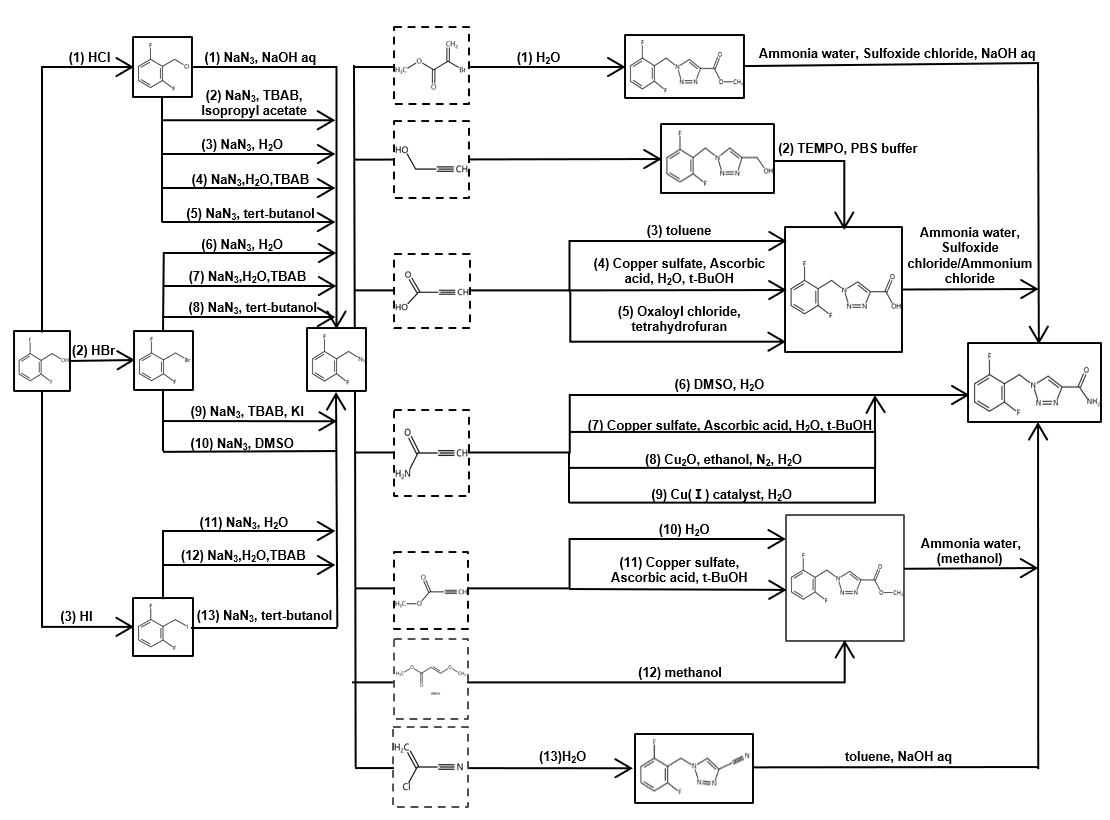
\includegraphics[width=1.1\linewidth]{superstructure1.png}
  \caption*{超结构示意图中的节点即边内的虚线框分别是合成主要物料的结构式,每条边对应一种具体合成路径}
  \caption{超结构模型示意图}
  \label{fig:superstructure}
\end{figure}

对于第一步卤化反应,在数据整理过程中我们发现针对三种主流卤化试剂(氯化氢、溴化氢、碘化氢)均有经过工艺研发者优化的合适的反应条件,且可以适用于连续反应,因此为了降低模型中不必要的复杂度,我们使用了一处贪心策略,在第一步中已经选取了各方面工艺参数都局部最优的三条路径纳入超结构中。值得注意的是,每种卤化试剂都选取了一条备择路径,无论优化决策结果如何,这并不代表其他试剂选择不存在拥有更优的合成路径的可能。这是由于缺乏足够的实验数据和机理模拟的手段,本工作在概念设计阶段无法直接对单步反应工艺在开发源头进行优化。

第二步叠氮化反应对第一步底物的适应性均较好,只是在最优操作条件方面有出入,在该步骤我们选取了所有可能的工艺组合共13种。本步骤中各工艺在溶剂选择方面存在较大差异,因此对反应体系的温度需求、操作需求和设备选型有一定影响。反应完成之后存在一步控温连续萃取操作,由于目标产物相同,该操作未包含在超结构内,但是纳入了对结构选型的优化的考量中。

第三步通过叠氮参与的1,3-偶极环加成反应生成相应的最终产物或前驱体,由于环加成反应过程中的极性中心处于优势区位,因此通常可以与亲核水解胺化等反应串联或一锅进行,是常见的有机连续合成策略。针对环加成过程,有两种反应机理,分别对应炔烃和烯醇类似底物,后者包含N-O的次级轨道相互作用,增强了烯醇类似底物的化学活性,因此拓展了反应的搜索空间\cite{paz2018}。图\ref{fig:superstructure}中对第三步反应的转化过程做了更详细的展示,共13种纳入考虑的合成路径。第三步中涉及的各个反应工艺的定制化都较强,在模型的数据准备中分别做了相应的考虑和计算,这为超结构模型的建立带来了形式上的统一。

\section{模型优化目标及约束}
\label{section:model}
\subsection{模型假设}

在建立超结构设计模型时,本文做出如下假设,在不失模型效力和不违背生产规律的前提下帮助模型尽可能得到有益的简化。

第一,假设各种所需物料的价格是定值,在生产过程中可以稳定获取不发生波动。本条假设是在调研了相关化学品近年的市场价格变动情况与数据丰富程度之后做出的。

第二,针对任一生产路径,不核算上游原材料及所有涉及物流的运输及仓储成本。

第三,假设所有超结构包含的合成路径在生产技术条件上是可行的,即未考虑由于工厂选址、地区因素,政策或环境因素引起的不支持特定操作要求和生产安排的情况,且生产装置在建设时已经充分考虑到为不确定性实现预留的操作空间。

第四,假设各生产路径的反应转化率是定值。本条假设要求反应条件在生产过程中的精准控制,应对催化剂更换或设备检修的详尽计划,由于这些工作是在概念设计阶段之后开展的,本文暂不考虑。

第五,假设使用的管式流动微反应器是完美数量放大的。本条假设要求所有的流动微反应器在制造和操作条件控制方面达到一致,因此产能可以呈整数倍数进行放大。这在设计阶段是合理的,并由此产生了追索问题的混合整数设计变量。

第六,对于固定投资的计算,假设其与设备操作量(对于本模型中通常按操作容积计)成正比,并按照设备购进价格按折旧率折算年费。

第七,对于操作成本的计算,假设公用工程费用以设计变量和参数的线性函数折算,对于能量消耗项的估算,认为与操作温度和室温的差成正比。

\subsection{成本函数}

如前所述,卢非酰胺的合成超结构优化主要以生产成本核算为优化目标。经济评估的目标往往是多方面的,为了模型的简明性和可解释性,在化工过程的概念设计过程中往往应用线性加合的方式构造单目标的成本函数\cite{yeoman1999,gong2017,madenoor2018},本模型的成本主要考虑选择相应工艺组合的年平均生产成本,包括以下各个部分。

第一,物料成本(Material Expenditure, $\symbfup{ME}$),如式\eqref{eq:me}。首先通过化学品交易平台数据库等获取,价格以美元计算;然后根据物料种类不同进行数据处理,具体而言,对于有明确投料比的合成原料或助剂,按照生产单位摩尔产物折算价格因子$c$;对于催化剂或可循环溶剂等,按照文献推测的更换频率,同样折算为生产单位摩尔产物的价格;对于一般的流动载体介质考虑在操作成本的溶剂回收项中。
\begin{align}
  \symbfup{ME} = \frac{\sum_{s}\symbfit c_s^T\symbfit X_s}{M_{\rm ruf}} \label{eq:me}
\end{align}
其中$s$为合成步骤的集合下标。

第二,固定成本(Capital Expenditure,$\symbfup{CE}$),如式\eqref{eq:ce}。固定成本投资只考虑了微反应器设备组件的资产投入\cite{diab2018,borukhova2016},按照连续药物分子合成工业设计的惯例,采用了按照标准设备投资($CE_0=374,600$美元)乘以容积因子\cite{diab2019}的方法估算。年费折旧率当开工时间$\symbfit\tau$不小于7000小时时按照全年8000小时计算,小于7000小时时按照近似的经验公式$\epsilon=15\%\times(1-\frac{\symbfit\tau}{8000})^{0.5}$计算\cite{baasal1989}。
\begin{align}
  \symbfup{CE} = \frac{\epsilon CE_0}{80.00}\sum_{s}\symbfit N_s\symbfit V_s \label{eq:ce}
\end{align}
其中$\symbfit N_s$表示设备台数,$\symbfit V_s$代表操作容积。

第三,操作成本(Operational Expenditure,$\symbfup{OE}$),如式\eqref{eq:oe}。操作成本项考虑了溶剂分离和处理操作的成本与电加热设备的能量消耗对应的公用工程支出,此处我们参考\cite{diab2018}的工作,按照系数折算法\cite{garrett2012}对两项成本进行估算,目的是为了考虑各个路径工艺选择在操作成本上的影响,以达到综合经济与环境因素影响的评估。
\begin{align}
  \symbfup{OE} = \sum_s \big(\xi\symbfit\tau_s(T_s-T_0)\symbfit N_s\symbfit L_s +E_{\rm rec}(1-r_{\rm rec})\symbfit N_s\symbfit L_s\symbfit V_s\big) \label{eq:oe}
\end{align}
其中各参数符号含义见表\ref{tab:notation},详细的计算方法在\ref{section:shebei}节中阐述。

\subsection{物料守恒}

引入变量$\symbfit X_s$对各个生产步骤的产能(即一年时间内该步主产物的总摩尔流量)进行描述,因此涉及到对每步步骤间的转化率进行核算,转化率采用基于上步产物纯品投料为基准计算,由于涉及到单程转化率、产率、分离比率等工艺细节问题,在物料衡算方面每步用统一的$\symbfit r_s$描述最终转化为该步产物纯品的表观产率,然后根据文献对工艺开发的描述和计算推测,根据单程转化时间$\symbfit \tau_s$的大小来反映若选择性和转化率低导致的额外分离对生产效能的影响。最终,第三步反应结束的后的产品卢非酰胺的目标用$PT$,以质量计的年生产目标这一超参数来约束。基于以上建模手段,物料守恒的约束为式\eqref{eq:mb1}-\eqref{eq:mb2}。
\begin{align}
  \symbfit X_0\sum_{i\in\mathbb I}\symbfit Y_i\symbfit r_i&=\sum_{i\in\mathbb I}\symbfit X_i \label{eq:mb1} \\
  \sum_{i\in\mathbb I}\symbfit X_i\sum_{j\in\mathbb J}\symbfit Y_j\symbfit r_j&=\sum_{j\in\mathbb J}\symbfit X_j \\
  \sum_{j\in\mathbb J}\symbfit X_j\sum_{k\in\mathbb K}\symbfit Y_k\symbfit r_k&=\sum_{i\in\mathbb K}\symbfit X_k \\
  \sum_{k\in\mathbb K}\symbfit X_kM_{\rm ruf}&\ge PT \label{eq:mb2}
\end{align}

\subsection{设备设计}
\label{section:shebei}

设备设计是本模型第二阶段的重要决策问题,主要问题在于规划合适的流动微反应器设备数量从而达到生产要求。流动微反应器因为拥有更强的传质传热能力,相比间歇反应的生产设备耗费人力更少,容易控制稳定的产品,而且也从某种程度上降低了设备占用规划、排班的设计难度,便于管理。对于一台流动反应设备,在给定的反应动力学和产物转化率的情况下,可以根据式\eqref{eq:lhsv}定义设备的液时空速$\symbfup {LHSV}$。
\begin{align}
  \symbfup{LHSV} = \left(\int_{X_{\rm in}}^{X_{\rm out}}\frac{\mathrm{d}X}{-\mathcal{r}_{\rm reaction}}\right)^{-1} \label{eq:lhsv}
\end{align}
式中$X_{\rm in}$和$X_{\rm out}$表示进入反应器与流出反应器的产物B浓度占投料A浓度的比率,$-\mathcal{r}_{\rm reaction}$表示由A生成B的动力学速率。其意义代表单位小时内被流动微反应器所处理的反应体系的总体积占反应器体积的比率。因此,对于模型中任一阶段反应的反应器操作体积为$\symbfit V_s$,操作时间为$t_{\rm opr}$,由相应的液时空速数据可以得到反应器设备与产能的关系为:
\begin{align}
  X_s = \symbfup{LHSV}_s\times\symbfit N_s\symbfit V_s\times t_{\rm{opr},s} \label{eq:equip1}
\end{align}

但是,在概念设计模型中,受到不同工艺的流程和后续处理差异较大的影响,$t_{\rm opr}$难以直接作为参数或变量出现。$\symbfup{LHSV}$是一个和操作条件、本征反应动力学、流动状态和催化剂填充状态相关的量,除了直接实验测定以外较难有精确的理论预测方式,因此,在设备设计部分我们采用如下的思路,通过文献的数据规模下的反推我们可以得出在一个操作步骤的总时长$\symbfit \tau_s$下产品的质量,由此我们定义“质量空速”($\symbfup{SV}_s$)为单位操作总时长下获得产品的质量,并定义新的决策变量$\symbfit L_s=\frac{t_{\rm{opr},s}}{\tau_s}$表示单套设备的处理量,因此设备与产能之间的关联式由式\eqref{eq:equip1}转化为\eqref{eq:equip2},即:
\begin{align}
  X_sM_{\rm ruf} = \symbfup{SV}_s\times\symbfit N_s\symbfit V_s\symbfit L_s\symbfit\tau_{s} \label{eq:equip2}
\end{align}
并将式\eqref{eq:equip2}中的参数合并定义为新的参数$\symbfup{SC}_s = \symbfup{SV}_s\symbfit V_s\symbfit\tau_{s}$。基于以上变量和参数的规定,达到生产要求的约束可以由操作时间导出:
\begin{align}
  \max\left\{\sum_{i\in\mathbb I}\symbfit L_i\symbfit\tau_i,\sum_{j\in\mathbb J}\symbfit L_j\symbfit\tau_j,\sum_{k\in\mathbb K}\symbfit L_k\symbfit\tau_k\right\} \le \tau^U
\end{align}
$\tau^U$是一个新的超参数,表示设备处在正常连续生产状态的总时间上限。

\section{逻辑约束}

超结构优化中的逻辑约束通常引入与决策维度相关的二元变量向量或矩阵来描述,最直观的一种表述就是“某个选项被选中/不被选中”分别对应二元变量“$\symbfit Y=1$/$\symbfit Y=0$”。对于本文模型,由于不需要类似STN网络中涉及多个任务类型的选取和转化,而是结构化地选取各步骤工艺路径,因此逻辑约束相对简单,如式\eqref{eq:lc1}-\eqref{eq:lc2}。其中$\symbfup M=10^5$为一个足够大的常量。
\begin{align}
  \sum_{i\in\mathbb I}\symbfit Y_i&=1 \label{eq:lc1} \\
  \sum_{j\in\mathbb J}\symbfit Y_j&=1 \\ 
  \sum_{k\in\mathbb K}\symbfit Y_k&=1 \\
  \symbfit X_s &\le \symbfup M\symbfit Y_s,\ \forall s\in \mathbb S = \mathbb I \cup\mathbb J\cup\mathbb K \label{eq:lc2} 
\end{align}

\section{确定性模型评估}
\subsection{确定性模型}

根据\ref{section:model}节的准备,本文构建的超结构优化模型的完整数学形式如式\eqref{eq:model1}-\eqref{eq:model2}所示。
\begin{align}
  \min_{\symbfit{X,Y,N}}\quad & \symbfup{ME} + \symbfup{CE} + \symbfup{OE} \label{eq:model1} \\
  s.t.\ \symbfup{ME} &= \frac{\sum_{s}\symbfit c_s^T\symbfit X_s}{M_{\rm ruf}} \\
   \symbfup{CE} &= \frac{\epsilon CE_0}{80.00}\sum_{s}\symbfit N_s\symbfit V_s \\
   \symbfup{OE} &= \sum_s \big(\xi\symbfit\tau_s(T_s-T_0)\symbfit N_s\symbfit L_s +E_{\rm rec}(1-r_{\rm rec})\symbfit N_s\symbfit L_s\symbfit V_s\big) \\
   X_sM_{\rm ruf} &= \symbfup{SV}_s\times\symbfit N_s\symbfit V_s\symbfit L_s\symbfit\tau_{s} \\
   &\symbfit X_0\sum_{i\in\mathbb I}\symbfit Y_i\symbfit r_i=\sum_{i\in\mathbb I}\symbfit X_i \\
  \sum_{i\in\mathbb I}&\symbfit X_i\sum_{j\in\mathbb J}\symbfit Y_j\symbfit r_j=\sum_{j\in\mathbb J}\symbfit X_j \\
  \sum_{j\in\mathbb J}&\symbfit X_j\sum_{k\in\mathbb K}\symbfit Y_k\symbfit r_k=\sum_{i\in\mathbb K}\symbfit X_k \\
  \sum_{k\in\mathbb K}&\symbfit X_kM_{\rm ruf}\ge PT \\
  \max&\left\{\sum_{i\in\mathbb I}\symbfit L_i\symbfit\tau_i,\sum_{j\in\mathbb J}\symbfit L_j\symbfit\tau_j,\sum_{k\in\mathbb K}\symbfit L_k\symbfit\tau_k\right\} \le \tau^U \\
  \sum_{i\in\mathbb I}\symbfit Y_i&=1  \\
  \sum_{j\in\mathbb J}\symbfit Y_j&=1 \\ 
  \sum_{k\in\mathbb K}\symbfit Y_k&=1 \\
  \symbfit X_s &\le \symbfup M\symbfit Y_s,\ \forall s\in \mathbb S = \mathbb I \cup\mathbb J\cup\mathbb K \label{eq:model2}
\end{align}

确定性模型包含连续变量126个,二元变量29个,整数变量29个,是一个MINLP模型。模型中各符号的含义整理在表\ref{tab:notation}中。

\begin{longtable}{cc}
  \caption{本文超结构优化模型的符号释义表}
  \label{tab:notation} \\
  \toprule
  参数或变量符号 & 含义 \\
  \midrule
\endfirsthead
  \caption*{续表~\thetable\quad 本文超结构优化模型的符号释义表} \\
  \toprule
  参数或变量符号 & 含义 \\
  \midrule
\endhead
  \bottomrule
\endfoot
$\mathbb I$ & 第一步反应路径选择的下标集合 \\
$\mathbb J$ & 第二步反应路径选择的下标集合 \\
$\mathbb K$ & 第三步反应路径选择的下标集合 \\
$\mathbb S$ & 所有反应路径选择的下标集合 \\
$\symbfit c_s$ & 某路径单位摩尔产物的物料价格因子 \\
$\symbfit V_s$ & 某路径选用设备的操作容积 \\
$\symbfit\tau_s$ & 某路径得到单位质量的该步产物所需操作的时间\\
$\symbfit r_s$ & 某路径投料转化为产品纯品的表观转化率\\
$T_s$ &  某路径的操作温度\\
$M_{\rm ruf}$ & 卢非酰胺分子的摩尔质量\\
$\epsilon$ &  流动微反应器设备的年平均折旧率\\
$\symbfup{SV}_s$ & 某路径下采用流动反应的“质量空速” (详细定义见\ref{section:shebei}节)\\
$CE_0$ & 标准单套设备投资\\
$E_{\rm rec}$ & 单位体积的溶剂消耗支出\\
$r_{\rm rec}$ & 溶剂回收率\\
$\xi$ & 公用工程成本折算系数\\
$T_0$ & 操作环境的室温\\
$\tau^U$ & 一年内设备处于正常生产状态的总时间上限\\
$PT$ & 一年内卢非酰胺的生产目标(按质量计)\\
$\symbfit X_0$ & 二氟苯甲醇前驱体的总需求量(以摩尔数计)\\
$\symbfit X_i$ & 第一步骤产品的预期总产能(以摩尔数计)\\
$\symbfit X_j$ & 第二步骤产品的预期总产能(以摩尔数计)\\
$\symbfit X_k$ & 第三步骤产品的预期总产能(以摩尔数计)\\
$\symbfit Y_s$ & 某路径是否选择的决策变量\\
$\symbfit N_s$ & 某路径选择下需要的设备数量\\
$\symbfit L_s$ & 某路径下流动反应器的年生产能力(详细定义见\ref{section:shebei}节)\\
\end{longtable}

\subsection{确定性模型求解结果}

本节中对确定性模型\eqref{eq:model1}-\eqref{eq:model2}的求解采用GAMS 34.2.0编写程序并用BARON求解器\cite{kilinc2018}求解,计算所用个人电脑的配置资源如下:处理器型号Intel® CoreTM i7-10175H(基准速度2.59GHz), 内存16GB,采用全部线程求解。

确定性模型采用的超参数标称点(Nominal Point)的值分别为:年生产目标$PT=100$kg,生产时间上限$\tau^U=7000$h,公用工程成本折算系数$\xi=4.525\times10^{-1}$,标称点参数的选取参考了以往发表的相关市场分析,模型与评估工作\cite{diab2018, padmaja2018},求解得到了确定性模型下成本最优的卢非酰胺连续合成路线:第一步反应采用溴化氢作为卤代试剂,第二步采用了无溶剂策略的重氮化反应\cite{gelonch2019},第三步反应采用了以DMSO为有机溶剂体系下的热催化Huisgen环加成反应。具体的路径结构采用红色高亮标注在图\ref{fig:deterministic}中。

\begin{figure}[ht!]
  \centering
  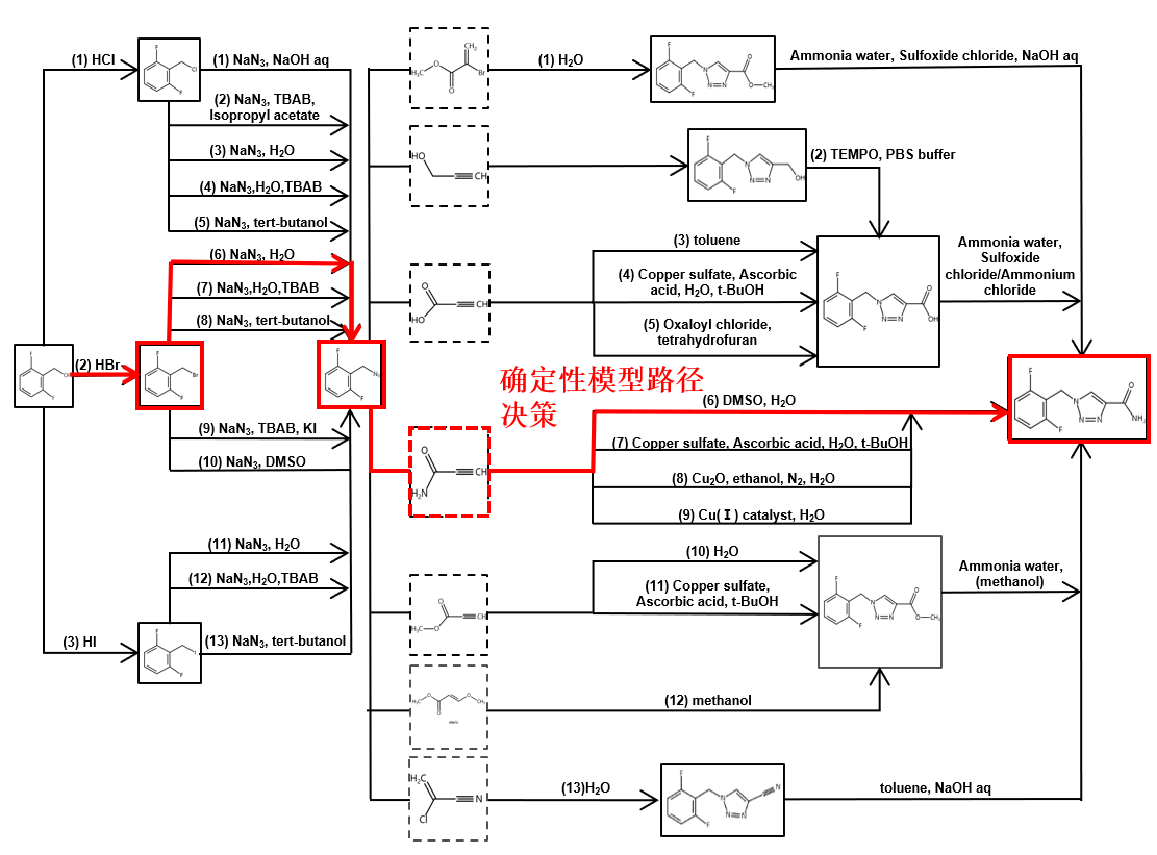
\includegraphics[width=1.1\linewidth]{deterministic.png}
  \caption{确定性模型最优超结构路径选择图示}
  \label{fig:deterministic}
\end{figure}

确定性模型的求解结果总结在下面表\ref{tab:deterministic}中。将目标函数中$\symbfup{ME}$、$\symbfup{CE}$及$\symbfup{OE}$的两项的计算结果用饼图\ref{fig:composition}表示,与已发表的关于卢非酰胺合成过程的经济评估的文献\cite{diab2018}进行对比,可以进一步验证模型的合理性。

\begin{figure}[ht!]
  \centering
  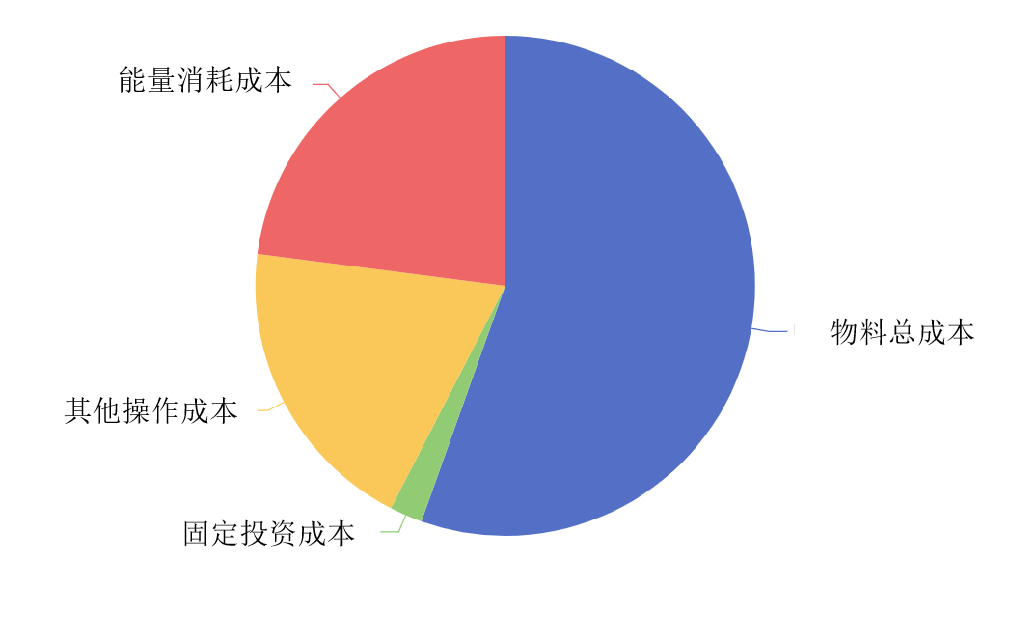
\includegraphics[width=12cm]{composition.png}
  \caption{确定性模型最优决策下成本函数的构成}
  \label{fig:composition}
\end{figure}

\begin{table}[ht!]
  \centering
  \begin{threeparttable}[c]
    \caption{卢非酰胺连续合成超结构确定性模型优化结果}
    \label{tab:deterministic}
    \begin{tabular}{cccccc}
      \toprule
       & 路径\tnote{1} & 设备需求量$\symbfit N_s$ & 总产量($\symbfit X_s$/mol) & 总产能\tnote{2}(kg)& 目标函数值(美元/年) \\
      \midrule
      步骤一 & 2   &  4   &  360.36	 &  74.60   &  \multirow[c]{3}{*}{$7.818\times 10^6$} \\
      步骤二 & 6   &  2   &  360.33	 &  60.93   & \\
      步骤三 & 6   &  32  &  353.12	 &  100.00  & \\
      \bottomrule
    \end{tabular}
    \begin{tablenotes}
      \item [1] 此处的数字表示各步骤备选路径所对应集合$\mathbb{I,J,K}$的下标$i,j,k$,后文中也用类似“2-6-6”的表述指代特定的路径决策组合。
      \item [2] 总产能即指当前路径设计下一年的生产周期内每个步骤预计产出的产品质量。
    \end{tablenotes}
  \end{threeparttable}
\end{table}

确定性模型的问题规模由表\ref{tab:problemscale}给出,该问题规模对于后续不确定性模型的构建有重要的影响。如果确定性模型问题规模过大,则会超出目前通用求解器所采用算法的上限,这是由于大规模问题的迭代算法的求解仍然是一个尚未完全解决的难题。

\begin{table}[ht!]
  \centering
  \caption{超结构优化确定性模型问题规模}
  \begin{tabular}{cccc}
    \toprule
    约束数量         & 单变量个数   &  非零变量个数   &  离散变量个数  \\
    \midrule
    141   & 125  &   497  &   58 \\
    \bottomrule
  \end{tabular}
  \label{tab:problemscale}
\end{table}

\section{不确定性优化模型}

不确定优化模型的构建是本文研究的重点,合理的不确定优化模型需要仔细考虑不确定因素的来源和参数化描述,不确定参数的集合表示形式与模型嵌入方式,然后选取合适的不确定优化决策模型。在本文构建的两阶段模型中,不确定参数主要来自生产规划的早期概念设计阶段,因此我们筛选路径阶段的决策主要来自于对具有表现出最大生产灵活性潜力的工艺路径的确定。然而,生产场景的不确定性直接关系到路径确定下过程设计决策的约束,因此需要根据不确定性的实现情况进行调整,在这个意义上,设计阶段自然成为第二阶段决策。因此,本文认为基于超结构优化模型的连续合成制备高附加值化学品的工艺综合与概念设计工作同两阶段的ARO框架有深远的一致性,两者分别是化学工业学科的研究场景与不确定优化方法的研究场景,其本质关联值得进一步探索。

\subsection{灵敏度分析与不确定参数选取}

模型对参数的灵敏度分析通常指通过在一定步长下逐参数选择地绘制模型输出对参数变化的响应特性,来发现特定参数对模型表现的影响,这在不确定性分析、模型诊断或基于信赖域的优化方法领域均有重要应用。对于确定性模型的超参数灵敏度分析主要通过对超参数进行赋值并求解出各个参数值下对应的最优路径和目标函数值。伴随着最优路径的变化,目标函数值对参数值的响应曲线呈现出拐点。

\begin{figure}
  \centering
  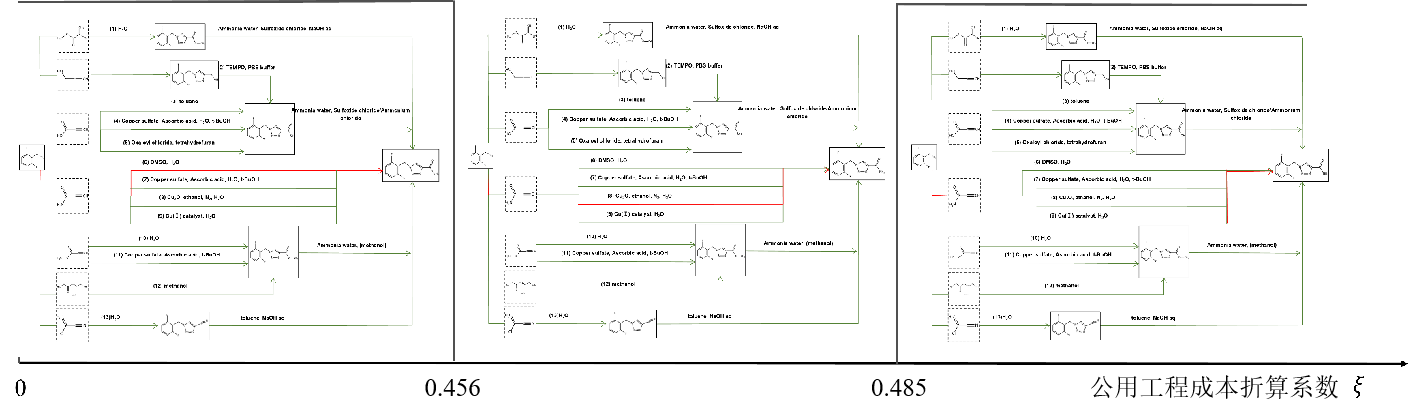
\includegraphics[width=1.1\linewidth]{xi.png}
  \caption{对超参数$\xi$的灵敏度分析示意图}
  \label{fig:xi}
\end{figure}

首先,在模型求解时固定确定性模型最优结构决策组合2-6-6,对于年生产目标$PT$超参数从50到600按步长为10依次取值,求解得到最优的目标函数随$PT$的变化曲线如图\ref{fig:pt}所示,可以看出,当前路径最大年生产能力可以达到550kg,这与已有文献\cite{gelonch2019}接近。取消对结构决策变量的固定取值,可以得到不同的年生产目标对应的最优路径选取也不同。另一个典型的例子是公用工程成本折算系数$\xi$,在标称点附近的波动范围内存在两个临界点。在$\xi\in\left[0.428,0.489\right]$范围内以$10^{-3}$为步长进行灵敏度分析,如图\ref{fig:xi}所示,在$\xi<0.456$时最优路径决策组合为2-6-6,当$0.456\le\xi<0.485$时最优解变为2-6-8,当$\xi\ge0.485$时变为2-6-9。

在最终的超结构不确定优化模型中,综合考虑灵敏度分析结果与参数意义,选取了$PT$、$\tau^U$和$\xi$三个不确定参数作为建立模型的基础。其中,考虑市场需求的不确定波动在药物等化学品制造的概念设计中经常引入\cite{pisti1995}。因此,卢非酰胺的药物API年生产目标可能会随市场预期或企业的产品结构调整而存在一定变化,然而,较大幅度的生产负荷波动在实际生产中并不现实,因此,我们考虑$PT$在$[50,150]$(kg)范围内波动。另外,考虑到新冠疫情爆发等大型公共事件对生产正常状况带来的影响,连续生产过程需要考虑由于停车、检修设备或应对突发状况而导致的生产周期缩短,因此在工艺与设备设计中往往要求一定的生产空间弹性以备预期生产目标的达成。因此,本文考虑设备正常运行的总时间上限$\tau^U$的标称值为7000小时,略低于一般生产设计中常用的8000小时惯例,而将不确定参数波动的偏差值$\increment \tau^U=1000$h。公用工程成本折算系数的不确定性主要来自于工厂选址或能源价格自身的波动等,同时可能与相关政策变化相关,但变化范围相应较小,在本文中我们选取$\increment\xi=4.5\times10^{-2}$,即标称点值的10\%。

在不确定集的刻画方面,由于三个不确定变量可以认为相互独立地进行波动,因此不失一般性地采用最简单的箱型不确定集(Box uncertainty set),将标称点置于箱型不确定集的几何中心。箱型不确定集的保守程度相对较高,且最坏情况通常实现到顶点的极端情况。对于本文的模型而言,箱型不确定集的这一特性是可以接受的,且此处不确定集合的具体形式并不影响后续计算流程的有效性。


\subsection{两阶段ARO模型建立}

确定了不确定集之后,可以根据传统的SRO框架构建最基础的不确定优化模型,如式\eqref{eq:romodel1}-\eqref{eq:romodel2}所示。

\begin{align}
  \min_{\symbfit{X,Y,N}}\ \max_{\symbfit \Gamma} \quad & \symbfup{ME} + \symbfup{CE} + \symbfup{OE} \label{eq:romodel1} \\
  s.t.\ \symbfup{ME} &= \frac{\sum_{s}\symbfit c_s^T\symbfit X_s}{M_{\rm ruf}} \\
   \symbfup{CE} &= \frac{\epsilon CE_0}{80.00}\sum_{s}\symbfit N_s\symbfit V_s \\
   \symbfup{OE} &= \sum_s \big(\xi\symbfit\tau_s(T_s-T_0)\symbfit N_s\symbfit L_s +E_{\rm rec}(1-r_{\rm rec})\symbfit N_s\symbfit L_s\symbfit V_s\big) \\
   X_sM_{\rm ruf} &= \symbfup{SV}_s\times\symbfit N_s\symbfit V_s\symbfit L_s\symbfit\tau_{s} \\
   &\symbfit X_0\sum_{i\in\mathbb I}\symbfit Y_i\symbfit r_i=\sum_{i\in\mathbb I}\symbfit X_i \\
  \sum_{i\in\mathbb I}&\symbfit X_i\sum_{j\in\mathbb J}\symbfit Y_j\symbfit r_j=\sum_{j\in\mathbb J}\symbfit X_j \\
  \sum_{j\in\mathbb J}&\symbfit X_j\sum_{k\in\mathbb K}\symbfit Y_k\symbfit r_k=\sum_{i\in\mathbb K}\symbfit X_k \\
  \sum_{k\in\mathbb K}&\symbfit X_kM_{\rm ruf}\ge PT \\
  \max&\left\{\sum_{i\in\mathbb I}\symbfit L_i\symbfit\tau_i,\sum_{j\in\mathbb J}\symbfit L_j\symbfit\tau_j,\sum_{k\in\mathbb K}\symbfit L_k\symbfit\tau_k\right\} \le \tau^U \\
  \sum_{i\in\mathbb I}\symbfit Y_i&=1  \\
  \sum_{j\in\mathbb J}\symbfit Y_j&=1 \\ 
  \sum_{k\in\mathbb K}\symbfit Y_k&=1 \\
  \symbfit X_s &\le \symbfup M\symbfit Y_s,\ \forall s\in \mathbb S = \mathbb I \cup\mathbb J\cup\mathbb K \\
  PT &= PT_0 + \Gamma_1\increment PT,\ |\Gamma_1|\le 1, \Gamma_1\in\mathbb Z \\
  \tau^U &= \tau_0^U + \Gamma_2\increment \tau^U,\ |\Gamma_2|\le 1, \Gamma_2\in\mathbb Z \\
  \xi &= \xi_0 + \Gamma_3\increment\xi,\ |\Gamma_3|\le 1, \Gamma_3\in\mathbb Z \label{eq:romodel2}
\end{align}

其中,$PT_0=100(\mathrm{kg}), \tau^U_0 = 7000({\mathrm h}), \xi_0=4.525\times 10^{-1}$均表示标称值。然而,当前的SRO模型并没有一个好的求解框架可以让决策者通过优化设计得到应对不确定性的方案,因此,在式\eqref{eq:aro1}的启发下,我们可以将SRO模型转化为两阶段ARO模型,如式\eqref{eq:aromodel1}-\eqref{eq:aromodel2}。

\begin{align}
  \min_{\symbfit{Y}}\ 0 + \max_{\symbfit \Gamma}\ \min_{\symbfit{X,N}}\quad & \symbfup{ME} + \symbfup{CE} + \symbfup{OE} \label{eq:aromodel1} \\
  s.t.\ \symbfup{ME} &= \frac{\sum_{s}\symbfit c_s^T\symbfit X_s}{M_{\rm ruf}} \\
   \symbfup{CE} &= \frac{\epsilon CE_0}{80.00}\sum_{s}\symbfit N_s\symbfit V_s \\
   \symbfup{OE} &= \sum_s \big(\xi\symbfit\tau_s(T_s-T_0)\symbfit N_s\symbfit L_s +E_{\rm rec}(1-r_{\rm rec})\symbfit N_s\symbfit L_s\symbfit V_s\big) \\
   X_sM_{\rm ruf} &= \symbfup{SV}_s\times\symbfit N_s\symbfit V_s\symbfit L_s\symbfit\tau_{s} \\
   &\symbfit X_0\sum_{i\in\mathbb I}\symbfit Y_i\symbfit r_i=\sum_{i\in\mathbb I}\symbfit X_i \\
  \sum_{i\in\mathbb I}&\symbfit X_i\sum_{j\in\mathbb J}\symbfit Y_j\symbfit r_j=\sum_{j\in\mathbb J}\symbfit X_j \\
  \sum_{j\in\mathbb J}&\symbfit X_j\sum_{k\in\mathbb K}\symbfit Y_k\symbfit r_k=\sum_{i\in\mathbb K}\symbfit X_k \\
  \sum_{k\in\mathbb K}&\symbfit X_kM_{\rm ruf}\ge PT \\
  \max&\left\{\sum_{i\in\mathbb I}\symbfit L_i\symbfit\tau_i,\sum_{j\in\mathbb J}\symbfit L_j\symbfit\tau_j,\sum_{k\in\mathbb K}\symbfit L_k\symbfit\tau_k\right\} \le \tau^U \\
  \sum_{i\in\mathbb I}\symbfit Y_i&=1  \\
  \sum_{j\in\mathbb J}\symbfit Y_j&=1 \\ 
  \sum_{k\in\mathbb K}\symbfit Y_k&=1 \\
  \symbfit X_s &\le \symbfup M\symbfit Y_s,\ \forall s\in \mathbb S = \mathbb I \cup\mathbb J\cup\mathbb K \\
  PT &= PT_0 + \Gamma_1\increment PT,\ |\Gamma_1|\le 1, \Gamma_1\in\mathbb Z \\
  \tau^U &= \tau_0^U + \Gamma_2\increment \tau^U,\ |\Gamma_2|\le 1, \Gamma_2\in\mathbb Z \\
  \xi &= \xi_0 + \Gamma_3\increment\xi,\ |\Gamma_3|\le 1, \Gamma_3\in\mathbb Z \label{eq:aromodel2}
\end{align}

至此,模型建立的工作已经初步完成。值得注意的是,模型\eqref{eq:aromodel1}-\eqref{eq:aromodel2}的追索问题包含混合整数决策变量$\symbfit N$,因此需要设计特殊的求解流程来解决混合整数追索问题,将在第\ref{section:solution}章中详细介绍。对该两阶段ARO模型的求解也将提供本文模型的卢非酰胺连续合成过程最优设计。

% 若图或表中有附注,采用英文小写字母顺序编号,附注写在图或表的下方。
% 国外的期刊习惯将图表的标题和说明文字写成一段,需要改写为标题只含图表的名称,其他说明文字以注释方式写在图表下方,或者写在正文中。

% 如果一个图由两个或两个以上分图组成时,各分图分别以 (a)、(b)、(c)...... 作为图序,并须有分图题。
% 推荐使用 \pkg{subcaption} 宏包来处理, 比如图~\ref{fig:subfig-a} 和图~\ref{fig:subfig-b}。

% \begin{figure}
%   \centering
%   \subcaptionbox{分图 A\label{fig:subfig-a}}
%     {
\includegraphics[width=0.35\linewidth]{example-image-a.pdf}}
%   \subcaptionbox{分图 B\label{fig:subfig-b}}
%     {
\includegraphics[width=0.35\linewidth]{example-image-b.pdf}}
%   \caption{多个分图的示例}
%   \label{fig:multi-image}
% \end{figure}

% \section{表格}

% 表应具有自明性。为使表格简洁易读,尽可能采用三线表,如表~\ref{tab:three-line}。
% 三条线可以使用 \pkg{booktabs} 宏包提供的命令生成。

% \begin{table}
%   \centering
%   \caption{三线表示例}
%   \begin{tabular}{ll}
%     \toprule
%     文件名          & 描述                         \\
%     \midrule
%     thuthesis.dtx   & 模板的源文件,包括文档和注释 \\
%     thuthesis.cls   & 模板文件                     \\
%     thuthesis-*.bst & BibTeX 参考文献表样式文件    \\
%     \bottomrule
%   \end{tabular}
%   \label{tab:three-line}
% \end{table}

% 表格如果有附注,尤其是需要在表格中进行标注时,可以使用 \pkg{threeparttable} 宏包。
% 研究生要求使用英文小写字母 a、b、c……顺序编号,本科生使用圈码 ①、②、③……编号。

% \begin{table}
%   \centering
%   \begin{threeparttable}[c]
%     \caption{带附注的表格示例}
%     \label{tab:three-part-table}
%     \begin{tabular}{ll}
%       \toprule
%       文件名                 & 描述                         \\
%       \midrule
%       thuthesis.dtx\tnote{a} & 模板的源文件,包括文档和注释 \\
%       thuthesis.cls\tnote{b} & 模板文件                     \\
%       thuthesis-*.bst        & BibTeX 参考文献表样式文件    \\
%       \bottomrule
%     \end{tabular}
%     \begin{tablenotes}
%       \item [a] 可以通过 xelatex 编译生成模板的使用说明文档;
%         使用 xetex 编译 \file{thuthesis.ins} 时则会从 \file{.dtx} 中去除掉文档和注释,得到精简的 \file{.cls} 文件。
%       \item [b] 更新模板时,一定要记得编译生成 \file{.cls} 文件,否则编译论文时载入的依然是旧版的模板。
%     \end{tablenotes}
%   \end{threeparttable}
% \end{table}

% 如某个表需要转页接排,可以使用 \pkg{longtable} 宏包,需要在随后的各页上重复表的编号。
% 编号后跟表题(可省略)和“(续)”,置于表上方。续表均应重复表头。

% \begin{longtable}{cccc}
%     \caption{跨页长表格的表题}
%     \label{tab:longtable} \\
%     \toprule
%     表头 1 & 表头 2 & 表头 3 & 表头 4 \\
%     \midrule
%   \endfirsthead
%     \caption*{续表~\thetable\quad 跨页长表格的表题} \\
%     \toprule
%     表头 1 & 表头 2 & 表头 3 & 表头 4 \\
%     \midrule
%   \endhead
%     \bottomrule
%   \endfoot
%   Row 1  & & & \\
%   Row 2  & & & \\
%   Row 3  & & & \\
%   Row 4  & & & \\
%   Row 5  & & & \\
%   Row 6  & & & \\
%   Row 7  & & & \\
%   Row 8  & & & \\
%   Row 9  & & & \\
%   Row 10 & & & \\
% \end{longtable}



% \section{算法}

% 算法环境可以使用 \pkg{algorithms} 或者 \pkg{algorithm2e} 宏包。

% \renewcommand{\algorithmicrequire}{\textbf{输入:}\unskip}
% \renewcommand{\algorithmicensure}{\textbf{输出:}\unskip}

% \begin{algorithm}
%   \caption{Calculate $y = x^n$}
%   \label{alg1}
%   \small
%   \begin{algorithmic}
%     \REQUIRE $n \geq 0$
%     \ENSURE $y = x^n$

%     \STATE $y \leftarrow 1$
%     \STATE $X \leftarrow x$
%     \STATE $N \leftarrow n$

%     \WHILE{$N \neq 0$}
%       \IF{$N$ is even}
%         \STATE $X \leftarrow X \times X$
%         \STATE $N \leftarrow N / 2$
%       \ELSE[$N$ is odd]
%         \STATE $y \leftarrow y \times X$
%         \STATE $N \leftarrow N - 1$
%       \ENDIF
%     \ENDWHILE
%   \end{algorithmic}
% \end{algorithm}

%% !TeX root = ../thuthesis-example.tex

\chapter{求解方法与结果}

本章讨论含有混合整数追索的两阶段ARO的求解问题。混合整数追索问题由于其精确求解算法难以寻找,在许多以往的工作中在建模环节中被规避
,或采用适当的松弛与近似求解策略。然而,对于化工过程综合与优化问题,混合整数问题是广泛存在的,要求追索问题始终拥有连续的搜索空间,即第二阶段决策始终为连续变量会大大限制两阶段ARO在具体问题中的适用性与可解释性。因此,拓展混合整数追索的处理策略是一个ARO研究的关键问题。

\section{含有混合整数追索的两阶段ARO求解策略}
\label{section:solution}
首先,本文回顾在两阶段ARO问题的一般求解算法中获得成功的C\&CG算法流程并做适当讨论。

\subsection{列与约束生成算法}

列与约束生成算法(C\&CG)与传统的Benders分解方法不同,每次主问题-子问题迭代中,主问题都会增加一组追索变量,称为“列生成”(Column Generation),同时增加一项切平面约束。针对如式\eqref{eq:ccg1}--\eqref{eq:ccg2}的两阶段鲁棒优化问题:
\begin{align}
  \min_{\symbfit y}\quad &\symbfit c^T\symbfit y + \max_{\symbfit u\in\mathbb U} \min_{\symbfit x\in \mathit F(\symbfit y, \symbfit u)} \symbfit b^T \symbfit x \label{eq:ccg1}\\
   s.t.\ & \symbfit{Ay}\ge \symbfit a \\
   &  \symbfit G \symbfit x \ge \symbfit h - \symbfit E \symbfit y - \symbfit M \symbfit u\label{eq:ccg2}
\end{align}

原始的列与约束生成算法如算法\ref{alg:ccg}所示。
\label{section:ccg}

\begin{algorithm}
  \caption{求解\eqref{eq:ccg1}--\eqref{eq:ccg2}的C\&CG算法流程} \label{alg:ccg}
  \small
  \begin{algorithmic}
    \STATE{} 令 $LB=-\infty, UB=+\infty$ 和 $k = 0$
    \WHILE{TRUE}
    \STATE{} 求解下述主问题
    \begin{align}
      (\symbfup{MP})\min_{\symbfit{y,x},\eta}\quad & \symbfit c^T\symbfit y+\eta \\
      s.t.\ & \symbfit{Ay}\ge \symbfit a \\
      & \eta \ge \symbfit b^T\symbfit x^{l}, \forall 1\le l \le k \\
      & \symbfit G \symbfit x^l \ge \symbfit h - \symbfit E \symbfit y - \symbfit M \symbfit u_l^*, \forall 1\le l\le k \\
      &\symbfit y\in\mathbb Y, \symbfit x^l\in \mathbb X\subset\mathbb R_+^p\forall 1\le 1\le k
    \end{align}
    \STATE{} 获取最优解$(\symbfit y_{k+1}^*, \eta_{k+1}^*, \symbfit z^1, \dots, \symbfit z^k, \symbfit x^1, \dots, \symbfit x^k)$
    \STATE{} 更新$LB\leftarrow \symbfit c^T\symbfit y_{k+1}^*+\eta_{k+1}^*$
    \STATE{} 求解下列子问题
    \begin{align}
      (\symbfup{SP})& \mathcal{Q}(\hat{\symbfit y})=\max_{\symbfit u\in\mathbb U}\min_{x\in\mathbb X} \symbfit b^T\symbfit x \\
      s.t.\ & \symbfit G \symbfit x \ge \symbfit h - \symbfit E \symbfit{\hat{y}}  - \symbfit M \symbfit u
    \end{align}
    \STATE{} 更新$UB\leftarrow \min\{UB, \symbfit c^T\symbfit y_{k+1}^*+\mathcal Q(\symbfit y_{k+1}^*)\}$
      \IF{$UB-LB\le\varepsilon$}
        \STATE{} 当前$\symbfit y_{k+1}^*$为最优解,迭代终止。
      \ELSE[]
      \STATE{} 构造一列新变量$(\symbfit z^{k+1}, \symbfit x^{k+1})$,并向主问题增加下面各组约束:
      \begin{align}
        & \eta \ge \symbfit b^T\symbfit x^{k+1} \\
      & \symbfit G \symbfit x^{k+1} \ge \symbfit h - \symbfit E \symbfit y - \symbfit M \symbfit u_{k+1}^*, \forall 1\le l\le k \\
      &\symbfit y\in\mathbb Y, \symbfit x^l\in \mathbb X\subset\mathbb R_+^p\forall 1\le 1\le k
      \end{align}
      \STATE{} $k\leftarrow k+1$
      \ENDIF{}
    \ENDWHILE{}
  \end{algorithmic}
\end{algorithm}

上述算法比基于传统切平面的Benders分解方法在早期搜索阶段具有更高的计算效率\cite{zeng2013},因此现在被更广泛地应用于较大规模的ARO问题的精确求解。然而,上述流程对应用限制最严格的在于$\mathcal Q(\hat{\symbfit y})$的精确求解,对于$x\in\mathbb X\subset \mathbb R_+^p$的连续追索情形,用于在算法\ref{alg:ccg}中计算$\mathcal Q(\hat{\symbfit y})$的工具被称为“谕示机”(Oracle),通常是利用可调鲁棒对等问题的转化为可以通过其他梯度优化方法求取最优解的NLP子问题,因此,混合追索问题的谕示机的构造是富有挑战的。而且,对于常见的$\symbfit u\in\mathbb U$,在ARO问题迭代流程中主问题对应一个半无限规划问题,其收敛性的证明往往非常困难。所幸,列与约束生成算法在谕示机有能力寻找最差条件下的$\symbfit u^*$的前提下,其主问题上下界之间的收敛性已被证明\cite{zhao2011}。这启示我们将相应主问题的变量空间进行进一步分割,构造多层上下界以分别处理当前问题的混合追索问题。

\subsection{改进的三层问题求解流程}

参考\eqref{eq:ccg1}--\eqref{eq:ccg2}的形式,一般的含有整数追索的两阶段ARO可以表示为式\eqref{eq:miparo1}--\eqref{eq:miparo2}

\begin{align}
  \min_{\symbfit{y}\in\mathbb Y}\quad & \symbfit c^T\symbfit y+ \max_{\symbfit u\in\mathbb U}\min_{\symbfit{x,z}} \symbfit b^T\symbfit x + \symbfit d^T\symbfit z\label{eq:miparo1}\\
  s.t.\ & \symbfit{Ay}\ge \symbfit a \\
  & \symbfit G \symbfit x + \symbfit {Rz} \ge \symbfit h - \symbfit E \symbfit y - \symbfit M \symbfit u \\
  & \symbfit x\in \mathbb X\subset\mathbb R_+^p, \symbfit z\in\mathbb Z\subset\mathbb N_+^p \label{eq:miparo2}
\end{align}

在相关工作\cite{zhao2011,zeng2013,zhao2012}的启发下,我们假设整数追索变量$\symbfit z$是有界的。因此,$\symbfit z = \bigcup\{\symbfit z^r\}_{r=1}^{\mathcal R}$,其中$\mathcal R\le{\rm Card}(\{\symbfit z\in\mathbb N_+^p | \symbfup{dom\ \symbfit z}\})$,在这个前提下,\ref{section:ccg}节中算法\ref{alg:ccg}的子问题$(\symbfup{SP})$可以被转写为等价的有限约束数量的两层问题形式:

\begin{align}
  (\symbfup{SP^\prime})\ & \mathcal{Q}(\hat{\symbfit y})=\max \theta \\
  s.t.\ & \theta\le \symbfit d^T\symbfit z^r + \min_{\symbfit x^r\in\mathbb X}\{\symbfit b^T\symbfit x^r: \symbfit G \symbfit x^r +\symbfit R\symbfit z^r\ge \symbfit h - \symbfit E \symbfit{\hat{y}}  - \symbfit M \symbfit u \} \\& \forall 1\le r\le \mathcal R \\
  &\symbfit u\in\mathbb U
\end{align}

$\symbfup{SP^\prime}$可以通过KKT条件等价转化为单层形式:

\begin{align}
  (\symbfup{SP^\prime})\ & \mathcal{Q}(\hat{\symbfit y})=\max \theta \\
  s.t.\ & \theta\le \symbfit d^T\symbfit z^r + \symbfit b^T\symbfit x^r \\
  & \symbfit G \symbfit x^r +\symbfit R\symbfit z^r\ge \symbfit h - \symbfit E \symbfit{\hat{y}}  - \symbfit M \symbfit u, \forall 1\le r\le \mathcal R \\
  & \symbfit G^T\symbfit \pi^r \le \symbfit b, \forall 1\le r\le \mathcal R \\
  & \symbfit x^r(\symbfit G^T\symbfit \pi^r -\symbfit b) =0, \forall 1\le r\le \mathcal R\\
  & \symbfit \pi^r(\symbfit G \symbfit x^r +\symbfit R\symbfit z^r- \symbfit h +\symbfit E \symbfit{\hat{y}}+ \symbfit M \symbfit u) =0, \forall 1\le r\le \mathcal R \\ 
  &\symbfit u\in\mathbb U, \symbfit x^r\in\mathbb X\subset \mathbb R_+^p, \symbfit \pi^r\in\mathbb R_+^{p^\prime}, \forall 1\le r\le \mathcal R 
\end{align}

根据以上转化,我们可以采用单独的C\&CG算法循环来充当谕示机的作用。因此,本文建立的可以精确求解式\eqref{eq:miparo1}--\eqref{eq:miparo2}含有混合追索变量下子问题的$\mathcal Q(\hat{\symbfit y})$值的求解流程,如算法\ref{alg:nccg}所示。

\begin{algorithm}
  \caption{求解\eqref{eq:miparo1}--\eqref{eq:miparo2}的算法流程} \label{alg:nccg}
  \small
  \begin{algorithmic}
    \STATE{} 令 $LB=-\infty, UB=+\infty$ 和 $k = 0$
    \WHILE{TRUE}
    \STATE{} 求解下述主问题
    \begin{align}
      (\symbfup{MP})\min_{\symbfit{y,x},\eta}\quad & \symbfit c^T\symbfit y+\eta \\
      s.t.\ & \symbfit{Ay}\ge \symbfit a \\
      & \eta \ge \symbfit b^T\symbfit x^{l}, \forall 1\le l \le k \\
      & \symbfit G \symbfit x^l \ge \symbfit h - \symbfit E \symbfit y - \symbfit M \symbfit u_l^*, \forall 1\le l\le k \\
      &\symbfit y\in\mathbb Y, \symbfit x^l\in \mathbb X\subset\mathbb R_+^p\forall 1\le 1\le k
    \end{align}
    \STATE{} 获取最优解$(\symbfit y_{k+1}^*, \eta_{k+1}^*, \symbfit z^1, \dots, \symbfit z^k, \symbfit x^1, \dots, \symbfit x^k)$
    \STATE{} 更新$LB\leftarrow \symbfit c^T\symbfit y_{k+1}^*+\eta_{k+1}^*$
    \STATE{} 求解下列子问题
    \begin{align}
      (\symbfup{SP})& \mathcal{Q}(\hat{\symbfit y})=\max_{\symbfit u\in\mathbb U}\min_{x\in\mathbb X} \symbfit b^T\symbfit x \\
      s.t.\ & \symbfit G \symbfit x \ge \symbfit h - \symbfit E \symbfit{\hat{y}}  - \symbfit M \symbfit u
    \end{align}
    \STATE{} 更新$UB\leftarrow \min\{UB, \symbfit c^T\symbfit y_{k+1}^*+\mathcal Q(\symbfit y_{k+1}^*)\}$
      \IF{$UB-LB\le\varepsilon$}
        \STATE{} 当前$\symbfit y_{k+1}^*$为最优解,迭代终止。
      \ELSE[]
      \STATE{} 构造一列新变量$(\symbfit z^{k+1}, \symbfit x^{k+1})$,并向主问题增加下面各组约束:
      \begin{align}
        & \eta \ge \symbfit b^T\symbfit x^{k+1} \\
      & \symbfit G \symbfit x^{k+1} \ge \symbfit h - \symbfit E \symbfit y - \symbfit M \symbfit u_{k+1}^*, \forall 1\le l\le k \\
      &\symbfit y\in\mathbb Y, \symbfit x^l\in \mathbb X\subset\mathbb R_+^p\forall 1\le 1\le k
      \end{align}
      \STATE{} $k\leftarrow k+1$
      \ENDIF{}
    \ENDWHILE{}
  \end{algorithmic}
\end{algorithm}

\section{算例测试}

将算法\ref{alg:nccg}应用在一个含混合整数追索的两阶段ARO基准问题(Benchmarking Problem)中进行测试\cite{zhao2012}。考虑呼叫中心或诊所常见的员工轮岗排班问题(Rostering Problem),该优化问题要求要求在满足行业约束和服务需求的同时尽可能的降低运营成本。因此该案例考虑了两种类型的员工,分别为正式员工和兼职员工,兼职员工可以临时用来应对服务需求的波动变化,因此将兼职员工的安排问题设置为第二阶段决策问题。由此建立了一个两阶段可调的排班问题如下:

\begin{align}
  \min_{\symbfit x}\quad &\sum_i\sum_t c_{i,t}x_{i,t}+ \max_{\symbfit d}\min_{\symbfit{y,z,w}}\left(\sum_{j}\sum_t(f_{j,t}y_{j,t}+h_{j,t}z_{j,t})+\sum_tM_tw_t\right) \label{eq:roster1} \\
  s.t.\ & x_{i,t}+x_{i,t+1}+x_{i,t+2}\le 2, \forall i\le I, \forall t\le T-3 \label{eq:roster2}\\
  & l_i\le\sum_{t}x_{i,t}\le u_i, \forall i\le I \label{eq:roster3}\\
  & y_{j,t} + y_{j,t+1} \le 1, \forall j\le J, \forall t\le T-2 \label{eq:roster4}\\
  & a_j\le\sum_{t}y_{j,t}\le b_j, \forall j\le J \label{eq:roster5} \\
  & z_{j,t} \le Ny_{j,t}, \forall j\le J, \forall t\le T \label{eq:roster6} \\
  & N\sum_ix_{i,t}+\sum_{j}z_{j,t}+w_t\ge d_t, \forall t\le T \label{eq:roster7} \\
  & x_{i,t}, y_{j,t}\in\{0,1\}, z_{j,t}, w_t\ge0 \label{eq:roster8}
\end{align}

模型描述的问题背景较为显然,此处不再赘述。其中约束条件\eqref{eq:roster2}要求正式员工不能连续工作三个班次以上,式\eqref{eq:roster4}要求兼职员工不能连续工作两个班次以上,式\eqref{eq:roster3}和\eqref{eq:roster5}分别限制了正式员工和兼职员工调班次总数的上下限。式\eqref{eq:roster6}表示了兼职员工工作小时数的上限,式\eqref{eq:roster7}描述了工作需求与在班员工数量之间的约束关系,式\eqref{eq:roster8}定义了四个决策变量的取值范围。表\ref{tab:roster}中梳理了该模型中各参数和变量的含义,并对参数的取值或变量的类型做了说明。

\begin{longtable}{ccc}
    \caption{基准问题\eqref{eq:roster1}--\eqref{eq:roster8}中参数与变量符号释义及取值范围表}
    \label{tab:roster} \\
    \toprule
    参数 &  含义 & 取值范围\\
    \midrule
  \endfirsthead
    \caption*{续表~\thetable\quad 基准问题\eqref{eq:roster1}--\eqref{eq:roster8}中参数与变量符号释义及取值范围表} \\
    \toprule
    参数 &  含义 & 取值范围 \\
    \midrule
  \endhead
    \bottomrule
  \endfoot
  $c_{i,t}$ & 正式员工$i$的固定工资	& $[5,15]$中取固定值 \\
  $f_{j,t}$ & 兼职员工$j$的固定工资 & $[20,30]$中取固定值 \\	
  $h_{j,t}$ & 兼职员工$j$的每小时工资& $[4,8]$中取固定值 \\
  $M_t$ & 未满足的服务需求的单位惩罚成本	& $[40,50]$中取固定值\\
  $l_i$ &  正式员工$i$班次总数的下限  & $[4,8]$中取固定值 \\	
  $u_i$ &  正式员工$i$班次总数的上限& $[8,14]$中取固定值 \\
  $a_j$ &  兼职员工$j$班次总数的下限 & $[2,4]$中取固定值 \\	
  $b_j$ &  兼职员工$j$班次总数的上限 & $[4,6]$中取固定值\\	
  $N$ &  员工的最大工作小时数 &  $N=8$\\	
  $T$ &  模型考虑的班次总数  & $T=21$\\	
  $I$ &  正式员工的总人数   &  $I=12$\\	
  $J$ &  兼职员工的总人数	 &  $J=3$\\
  $x_{i,t}$ &  $t$班次内是否使用正式员工$i$ &	二元变量 \\
  $y_{j,t}$& $t$班次内是否使用兼职员工$j$	& 二元变量 \\
  $z_{j}$ & 兼职员工$j$的工作小时数	& 连续变量 \\
  $w_t$  & 未满足的服务需求小时数	& 连续变量 \\
  $d_t$  & 需求量	& 不确定性参数 \\
\end{longtable}

通过用Pyomo编程并通过GAMS调用CPLEX求解器求解这个该问题案例。原问题中包含316个整数二元决策变量,84个连续决策变量,609个约束条件和1个21维的不确定性参数集合。固定参数值采用随机选取的方法进行50次随机测试。合理设置模型的初始值,外层问题上下界迅速缩小,gap≤1\%左右时搜索较慢,但最终全部测试样例可以成功求解。图\ref{fig:roster}展示了在时的一次随机试验结果,此时,外层问题在迭代10次后模型的求解算法收敛到最优解。

\begin{figure}[ht!]
  \centering
  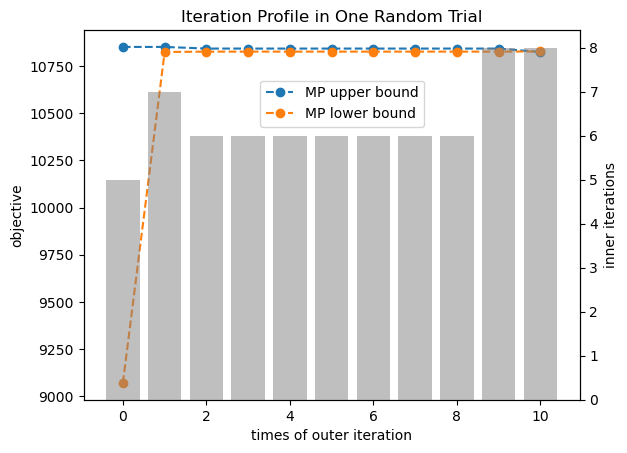
\includegraphics[width=0.8\linewidth]{roster.png}
  \caption{对算法\ref{alg:nccg}的某次基准问题测试收敛过程示意图}
  \label{fig:roster}
\end{figure}

因此,该求解流程可以有效求解一般的含有混合整数追索问题的ARO问题。

\section{本文不确定模型的求解}

本文的卢非酰胺连续合成超结构优化所建立的两阶段ARO模型适用于\ref{alg:nccg}的求解,具体转化与求解步骤见附录。下面着重探讨求解的结果。

\subsection{求解结果与分析}

本节中对模型\eqref{eq:aromodel1}-\eqref{eq:aromodel2}的求解采用GAMS 34.2.0编写程序并用BARON求解器\cite{kilinc2018}求解,计算所用个人电脑的配置资源如下:处理器型号Intel® CoreTM i7-10175H(基准速度2.59GHz), 内存16GB,采用全部线程求解。

经过计算得到的最优设计方案如表\ref{tab:rufiaro}所示。反应筛选到的最优设计路径方案为2-6-9,如图\ref{fig:rufiaro}所示。在三个反应步骤所设计采用的反应设备数量分别为7个、2个、4个,与确定性模型发生了较大的变化,另外,设计方案的最优目标函数为$1.198\times10^7$美元/年,相比确定性模型的结果提高了$53.3\%$左右,这是由于应对不确定性带来的成本提高,如预期生产规模的扩大、总时间上限的缩短和公用工程购买费用的提高。

\begin{table}[ht!]
  \centering
  \begin{threeparttable}[c]
    \caption{卢非酰胺连续合成超结构ARO模型优化结果}
    \label{tab:rufiaro}
    \begin{tabular}{cccccc}
      \toprule
       & 路径 & 设备需求量$\symbfit N_s$ & 总产量($\symbfit X_s$/mol) & 总产能(kg)& 目标函数值(美元/年) \\
      \midrule
      步骤一 & 2   &  7   &  557.61	 &  115.43   &  \multirow[c]{3}{*}{$1.198\times 10^7$} \\
      步骤二 & 6   &  2   &  557.56	 &  94.28   & \\
      步骤三 & 9   &  4  &  529.68	 &  150.00  & \\
      \bottomrule
    \end{tabular}
  \end{threeparttable}
\end{table}

\begin{figure}
  \centering
  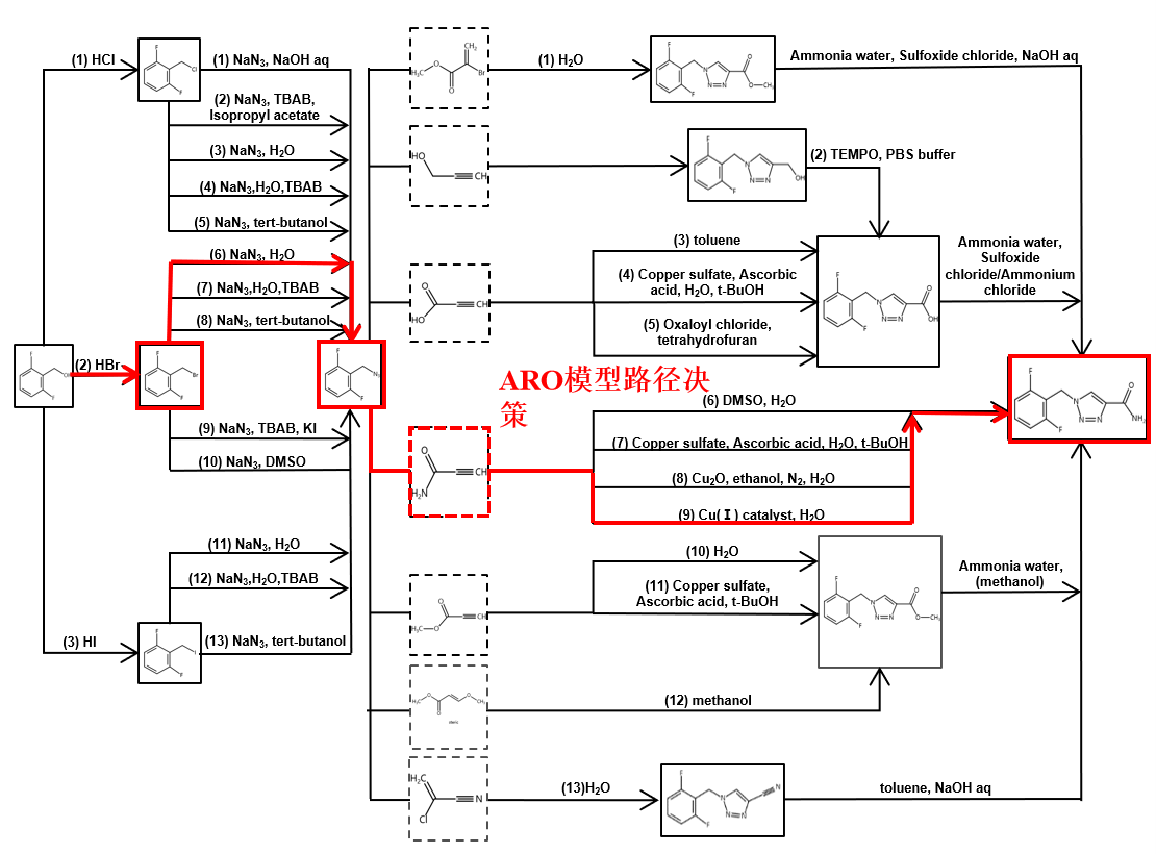
\includegraphics[width=1.1\linewidth]{ARO.png}
  \caption{ARO模型最优超结构路径选择图示}
  \label{fig:rufiaro}
\end{figure}

\subsection{不确定条件下的最优路径}

与确定性优化相比,ARO模型优化获得的求解路径发生改变,具体而言在本问题的模型中第三阶段的最优工艺路径选择发生改变。这说明在超结构优化中考虑不确定性参数的设计可能与不考虑不确定参数时拥有本质的不同,应对不确定性波动的能力更优的方案选择与在标称点下进行优化的最优方案选择不总是相同,这为决策者提供了另一种视角:过程抵抗不确定性波动的潜力与过程设计的预期成本之间存在一种博弈关系(Trade-off),决策者在概念设计阶段理性选择寻找二者之间的平衡点,是确定性模型与不确定性模型之间在模型解释性、参数响应性与最优决策的差异比较的关键作用。
在比较不确定性和确定性模型选出的最佳路径时,第一阶段和第二阶段得到的路径一致。然而,在第三阶段,不确定性模型选出了需要催化剂的路径9,而确定性模型则选出了成本更低的路径6,因为它不需要催化剂且原材料更经济。尽管如此,路径6在性能上不足以应对不确定性带来的挑战,这导致需要使用昂贵的一价铜催化剂来补偿。铜催化的叠氮-炔环加成反应是点击化学中一个典型例子,由诺贝尔奖得主K. Barry Sharpless提出,特点是高收率、广泛的应用、单一的副产物、立体选择性以及易于操作和溶剂去除。特别是,这个反应的速率比非催化的1,3-偶极环加成反应快100多倍。实验数据表明,在Cu(I)催化剂和水的体系下,卢非酰胺的一锅法合成过程可以达到95\%的最终收率,该结果说明了针对点击化学反应的研究与改进对高附加值化学品连续合成的工艺优化具有重要的潜在积极影响。

\subsection{鲁棒性检验}

本节对三种不确定性因素进行随机采样,随机选取50个不同的生产场景,讨论确定性优化方案和不确定性自适应可调鲁棒优化方案的样本外鲁棒性能。图\ref{fig:rotest}给出了确定性优化拓扑结构(2-6-6)和ARO优化拓扑结构(2-6-9)在上述50个场景下的成本效应。对比结果表明,两阶段ARO优化解析的拓扑结构能够以更低的成本应对随机场景,实现了鲁棒性能和经济性能更好的平衡。

\begin{figure}
  \centering
  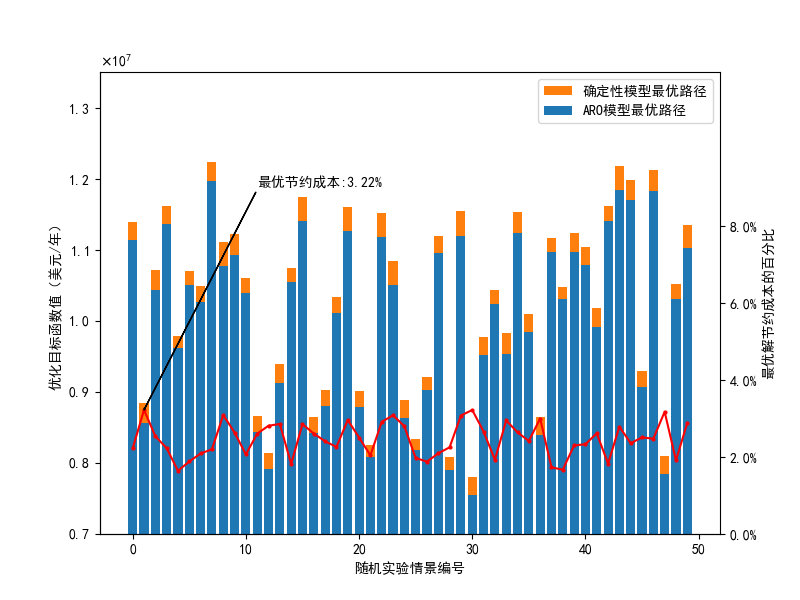
\includegraphics[width=\linewidth]{rotest.png}
  \caption{固定路径决策的确定性模型与ARO模型的随机试验目标函数对比}
  \label{fig:rotest}
\end{figure}



% % \section{数学符号}

% 中文论文的数学符号默认遵循 GB/T 3102.11—1993《物理科学和技术中使用的数学符号》
% \footnote{原 GB 3102.11—1993,自 2017 年 3 月 23 日起,该标准转为推荐性标准。}。
% 该标准参照采纳 ISO 31-11:1992 \footnote{目前已更新为 ISO 80000-2:2019。},
% 但是与 \TeX{} 默认的美国数学学会(AMS)的符号习惯有所区别。
% 具体地来说主要有以下差异:
% \begin{enumerate}
%   \item 大写希腊字母默认为斜体,如
%     \begin{equation*}
%       \Gamma \Delta \Theta \Lambda \Xi \Pi \Sigma \Upsilon \Phi \Psi \Omega.
%     \end{equation*}
%     注意有限增量符号 $\increment$ 固定使用正体,模板提供了 \cs{increment} 命令。
%   \item 小于等于号和大于等于号使用倾斜的字形 $\le$、$\ge$。
%   \item 积分号使用正体,比如 $\int$、$\oint$。
%   \item
%     偏微分符号 $\partial$ 使用正体。
%   \item
%     省略号 \cs{dots} 按照中文的习惯固定居中,比如
%     \begin{equation*}
%       1, 2, \dots, n \quad 1 + 2 + \dots + n.
%     \end{equation*}
%   \item
%     实部 $\Re$ 和虚部 $\Im$ 的字体使用罗马体。
% \end{enumerate}

% 以上数学符号样式的差异可以在模板中统一设置。
% 另外国标还有一些与 AMS 不同的符号使用习惯,需要用户在写作时进行处理:
% \begin{enumerate}
%   \item 数学常数和特殊函数名用正体,如
%     \begin{equation*}
%       \uppi = 3.14\dots; \quad
%       \symup{i}^2 = -1; \quad
%       \symup{e} = \lim_{n \to \infty} \left( 1 + \frac{1}{n} \right)^n.
%     \end{equation*}
%   \item 微分号使用正体,比如 $\dif y / \dif x$。
%   \item 向量、矩阵和张量用粗斜体(\cs{symbf}),如 $\symbf{x}$、$\symbf{\Sigma}$、$\symbfsf{T}$。
%   \item 自然对数用 $\ln x$ 不用 $\log x$。
% \end{enumerate}


% 英文论文的数学符号使用 \TeX{} 默认的样式。
% 如果有必要,也可以通过设置 \verb|math-style| 选择数学符号样式。

% 关于量和单位推荐使用
% \href{http://mirrors.ctan.org/macros/latex/contrib/siunitx/siunitx.pdf}{\pkg{siunitx}}
% 宏包,
% 可以方便地处理希腊字母以及数字与单位之间的空白,
% 比如:
% \SI{6.4e6}{m},
% \SI{9}{\micro\meter},
% \si{kg.m.s^{-1}},
% \SIrange{10}{20}{\degreeCelsius}。



% % \section{数学公式}

% 数学公式可以使用 \env{equation} 和 \env{equation*} 环境。
% 注意数学公式的引用应前后带括号,通常使用 \cs{eqref} 命令,比如式\eqref{eq:example}。
% \begin{equation}
%   \frac{1}{2 \uppi \symup{i}} \int_\gamma f = \sum_{k=1}^m n(\gamma; a_k) \mathscr{R}(f; a_k).
%   \label{eq:example}
% \end{equation}

% 多行公式尽可能在“=”处对齐,推荐使用 \env{align} 环境。
% \begin{align}
%   a & = b + c + d + e \\
%     & = f + g
% \end{align}



% % \section{数学定理}

% 定理环境的格式可以使用 \pkg{amsthm} 或者 \pkg{ntheorem} 宏包配置。
% 用户在导言区载入这两者之一后,模板会自动配置 \env{theorem}、\env{proof} 等环境。

% \begin{theorem}[Lindeberg--Lévy 中心极限定理]
%   设随机变量 $X_1, X_2, \dots, X_n$ 独立同分布, 且具有期望 $\mu$ 和有限的方差 $\sigma^2 \ne 0$,
%   记 $\bar{X}_n = \frac{1}{n} \sum_{i+1}^n X_i$,则
%   \begin{equation}
%     \lim_{n \to \infty} P \left(\frac{\sqrt{n} \left( \bar{X}_n - \mu \right)}{\sigma} \le z \right) = \Phi(z),
%   \end{equation}
%   其中 $\Phi(z)$ 是标准正态分布的分布函数。
% \end{theorem}
% \begin{proof}
%   Trivial.
% \end{proof}

% 同时模板还提供了 \env{assumption}、\env{definition}、\env{proposition}、
% \env{lemma}、\env{theorem}、\env{axiom}、\env{corollary}、\env{exercise}、
% \env{example}、\env{remar}、\env{problem}、\env{conjecture} 这些相关的环境。

%% % !TeX root = ../thuthesis-example.tex

\chapter{结论与展望}

本文建立了包含507中可能工艺路径的卢非酰胺连续合成过程超结构优化模型,并在不确定条件存在下通过两阶段可调鲁棒优化方法找到了最优路径选择,并设计了预期年成本投入1.2千万美元的最优合成过程。

本文针对卢非酰胺药物API分子的上游合成设计缺少概念设计、综合与不确定性优化结合的研究这一问题,利用已有的对卢非酰胺连续合成模式生产有应用潜力的工艺路径建立了基于超结构优化的过程综合与设计模型,在应对三种生产不确定性并存的情景下,采用了两阶段可调鲁棒优化方法建立了同时对工艺路径选择进行筛选和进行过程设计优化的两阶段模型。该模型的决策对生产不确定性有充分的应对能力,且可以识别出在不确定条件下更优的超结构决策,提供更大的生产设计空间。

为解决两阶段超结构优化模型中存在的混合整数追索问题,本文提出了一种改进的基于列与约束生成算法的求解流程,可以在不引入决策规则前提下精确求解含有混合整数追索的两阶段可调鲁棒优化问题。该计算流程的提出为两阶段模型的建立拓展了应用与研究的场景,使基于超结构优化的化工过程综合与设计优化模型拥有了更加广阔丰富的应用前景,

然而,与本文研究目标相关的课题仍然还有很多值得进一步探讨的内容。首先,从求解方法上来看,当前算法在规模不算太大的优化模型中尚有可接受的计算效率表现,然而对于更一般的化工过程设计问题,其求解效率仍然太低,而且灵活性不足,三层问题结构下算法流程的应用便利性和可扩展性也受到较大限制。未来更有效率的分解与剪枝策略,或基于学习策略的定制切平面方案与单纯应用列与约束生成算法的框架结合可能会提供更加高效与可扩展的含有混合整数追索的ARO求解算法。

其次,在模型方法上,本文对于卢非酰胺这一特定化学品生产目标的工艺综合与设计,问题本身存在一定场景局限性,在实际高端化学品生产工业中,往往面临着多条产线的并行、调度、联合生产,还有许多工业化生产场景的细节未能充分考虑,因此本文的模型相比实际落地还有较远的距离,简化程度仍然较高。为了更好地连接概念设计阶段与项目方案设计阶段,更详细的工艺细节开发与更全面的经济评估是下一步亟待开展的工作。






% 模板支持 BibTeX 和 BibLaTeX 两种方式处理参考文献。
% 下文主要介绍 BibTeX 配合 \pkg{natbib} 宏包的主要使用方法。


% \section{顺序编码制}

% 在顺序编码制下,默认的 \cs{cite} 命令同 \cs{citep} 一样,序号置于方括号中,
% 引文页码会放在括号外。
% 统一处引用的连续序号会自动用短横线连接。

% \thusetup{
%   cite-style = super,
% }
% \noindent
% % \begin{tabular}{l@{\quad$\Rightarrow$\quad}l}
%   \verb|\cite{zhangkun1994}|               & \cite{zhangkun1994}               \\
%   \verb|\citet{zhangkun1994}|              & \citet{zhangkun1994}              \\
%   \verb|\citep{zhangkun1994}|              & \citep{zhangkun1994}              \\
%   \verb|\cite[42]{zhangkun1994}|           & \cite[42]{zhangkun1994}           \\
%   \verb|\cite{zhangkun1994,zhukezhen1973}| & \cite{zhangkun1994,zhukezhen1973} \\
% \end{tabular}


% 也可以取消上标格式,将数字序号作为文字的一部分。
% 建议全文统一使用相同的格式。

% \thusetup{
%   cite-style = inline,
% }
% \noindent
% \begin{tabular}{l@{\quad$\Rightarrow$\quad}l}
%   \verb|\cite{zhangkun1994}|               & \cite{zhangkun1994}               \\
%   \verb|\citet{zhangkun1994}|              & \citet{zhangkun1994}              \\
%   \verb|\citep{zhangkun1994}|              & \citep{zhangkun1994}              \\
%   \verb|\cite[42]{zhangkun1994}|           & \cite[42]{zhangkun1994}           \\
%   \verb|\cite{zhangkun1994,zhukezhen1973}| & \cite{zhangkun1994,zhukezhen1973} \\
% \end{tabular}



% \section{著者-出版年制}

% 著者-出版年制下的 \cs{cite} 跟 \cs{citet} 一样。

% \thusetup{
%   cite-style = author-year,
% }
% \noindent
% \begin{tabular}{@{}l@{$\Rightarrow$}l@{}}
%   \verb|\cite{zhangkun1994}|                & \cite{zhangkun1994}                \\
%   \verb|\citet{zhangkun1994}|               & \citet{zhangkun1994}               \\
%   \verb|\citep{zhangkun1994}|               & \citep{zhangkun1994}               \\
%   \verb|\cite[42]{zhangkun1994}|            & \cite[42]{zhangkun1994}            \\
%   \verb|\citep{zhangkun1994,zhukezhen1973}| & \citep{zhangkun1994,zhukezhen1973} \\
% \end{tabular}

% \vskip 2ex
% \thusetup{
%   cite-style = super,
% }
% 注意,引文参考文献的每条都要在正文中标注
% \cite{zhangkun1994,zhukezhen1973,dupont1974bone,zhengkaiqing1987,%
%   jiangxizhou1980,jianduju1994,merkt1995rotational,mellinger1996laser,%
%   bixon1996dynamics,mahui1995,carlson1981two,taylor1983scanning,%
%   taylor1981study,shimizu1983laser,atkinson1982experimental,%
%   kusch1975perturbations,guangxi1993,huosini1989guwu,wangfuzhi1865songlun,%
%   zhaoyaodong1998xinshidai,biaozhunhua2002tushu,chubanzhuanye2004,%
%   who1970factors,peebles2001probability,baishunong1998zhiwu,%
%   weinstein1974pathogenic,hanjiren1985lun,dizhi1936dizhi,%
%   tushuguan1957tushuguanxue,aaas1883science,fugang2000fengsha,%
%   xiaoyu2001chubanye,oclc2000about,scitor2000project%
% }。



% 其他部分
\backmatter
% 插图和附表清单
% 本科生的插图索引和表格索引需要移至正文之后、参考文献前
% \listoffiguresandtables  % 插图和附表清单(仅限研究生)
%\listoffigures           % 插图清单
%\listoftables            % 附表清单

% 参考文献
\bibliography{ref/myrefs}  % 参考文献使用 BibTeX 编译
% \printbibliography       % 参考文献使用 BibLaTeX 编译

% 致谢
%% !TeX root = ../thuthesis-example.tex

\begin{acknowledgements}
  衷心感谢导师×××教授和物理系××副教授对本人的精心指导。他们的言传身教将使我终生受益。

  在美国麻省理工学院化学系进行九个月的合作研究期间,承蒙 Robert Field 教授热心指导与帮助,不胜感激。

  感谢×××××实验室主任×××教授,以及实验室全体老师和同窗们学的热情帮助和支持!

  本课题承蒙国家自然科学基金资助,特此致谢。
\end{acknowledgements}


% 声明
% 本科生开题报告不需要
% \statement
% 将签字扫描后的声明文件 scan-statement.pdf 替换原始页面
% \statement[file=scan-statement.pdf]
% 本科生编译生成的声明页默认不加页脚,插入扫描版时再补上;
% 研究生编译生成时有页眉页脚,插入扫描版时不再重复。
% 也可以手动控制是否加页眉页脚
% \statement[page-style=empty]
% \statement[file=scan-statement.pdf, page-style=plain]

% 附录
% 本科生需要将附录放到声明之后,个人简历之前
% \appendix
% % !TeX root = ../thuthesis-example.tex

\begin{survey}
\label{cha:survey}

\title{Title of the Survey}
\maketitle


\tableofcontents


本科生的外文资料调研阅读报告。


\section{Figures and Tables}

\subsection{Figures}

An example figure in appendix (Figure~\ref{fig:appendix-survey-figure}).

\begin{figure}
  \centering
  
\includegraphics[width=0.6\linewidth]{example-image-a.pdf}
  \caption{Example figure in appendix}
  \label{fig:appendix-survey-figure}
\end{figure}


\subsection{Tables}

An example table in appendix (Table~\ref{tab:appendix-survey-table}).

\begin{table}
  \centering
  \caption{Example table in appendix}
  \begin{tabular}{ll}
    \toprule
    File name       & Description                                         \\
    \midrule
    thuthesis.dtx   & The source file including documentation and comments \\
    thuthesis.cls   & The template file                                   \\
    thuthesis-*.bst & BibTeX styles                                       \\
    thuthesis-*.bbx & BibLaTeX styles for bibliographies                  \\
    thuthesis-*.cbx & BibLaTeX styles for citations                       \\
    \bottomrule
  \end{tabular}
  \label{tab:appendix-survey-table}
\end{table}


\section{Equations}

An example equation in appendix (Equation~\eqref{eq:appendix-survey-equation}).
\begin{equation}
  \frac{1}{2 \uppi \symup{i}} \int_\gamma f = \sum_{k=1}^m n(\gamma; a_k) \mathscr{R}(f; a_k)
  \label{eq:appendix-survey-equation}
\end{equation}


\section{Citations}

Example\cite{dupont1974bone} citations\cite{merkt1995rotational} in appendix
\cite{dupont1974bone,merkt1995rotational}.


% 默认使用正文的参考文献样式;
% 如果使用 BibTeX,可以切换为其他兼容 natbib 的 BibTeX 样式。
\bibliographystyle{unsrtnat}
% \bibliographystyle{IEEEtranN}

% 默认使用正文的参考文献 .bib 数据库;
% 如果使用 BibTeX,可以改为指定数据库,如 \bibliography{ref/refs}。
\printbibliography

\end{survey}
       % 本科生:外文资料的调研阅读报告
% % !TeX root = ../thuthesis-example.tex

\begin{translation}
\label{cha:translation}

\title{书面翻译题目}
\maketitle

\tableofcontents


本科生的外文资料书面翻译。


\section{图表示例}

\subsection{图}

附录中的图片示例(图~\ref{fig:appendix-translation-figure})。

\begin{figure}
  \centering
  
\includegraphics[width=0.6\linewidth]{example-image-a.pdf}
  \caption{附录中的图片示例}
  \label{fig:appendix-translation-figure}
\end{figure}


\subsection{表格}

附录中的表格示例(表~\ref{tab:appendix-translation-table})。

\begin{table}
  \centering
  \caption{附录中的表格示例}
  \begin{tabular}{ll}
    \toprule
    文件名          & 描述                         \\
    \midrule
    thuthesis.dtx   & 模板的源文件,包括文档和注释 \\
    thuthesis.cls   & 模板文件                     \\
    thuthesis-*.bst & BibTeX 参考文献表样式文件    \\
    thuthesis-*.bbx & BibLaTeX 参考文献表样式文件  \\
    thuthesis-*.cbx & BibLaTeX 引用样式文件        \\
    \bottomrule
  \end{tabular}
  \label{tab:appendix-translation-table}
\end{table}


\section{数学公式}

附录中的数学公式示例(公式\eqref{eq:appendix-translation-equation})。
\begin{equation}
  \frac{1}{2 \uppi \symup{i}} \int_\gamma f = \sum_{k=1}^m n(\gamma; a_k) \mathscr{R}(f; a_k)
  \label{eq:appendix-translation-equation}
\end{equation}


\section{文献引用}

附录\cite{dupont1974bone}中的参考文献引用\cite{merkt1995rotational}示例
\cite{dupont1974bone,merkt1995rotational}。


\appendix

\section{附录}

附录的内容。


% 书面翻译的参考文献
% 默认使用正文的参考文献样式;
% 如果使用 BibTeX,可以切换为其他兼容 natbib 的 BibTeX 样式。
\bibliographystyle{unsrtnat}
% \bibliographystyle{IEEEtranN}

% 默认使用正文的参考文献 .bib 数据库;
% 如果使用 BibTeX,可以改为指定数据库,如 \bibliography{ref/refs}。
\printbibliography

% 书面翻译对应的原文索引
\begin{translation-index}
  \nocite{mellinger1996laser}
  \nocite{bixon1996dynamics}
  \nocite{carlson1981two}
  \bibliographystyle{unsrtnat}
  \printbibliography
\end{translation-index}

\end{translation}
  % 本科生:外文资料的书面翻译
% % !TeX root = ../thuthesis-example.tex

\chapter{补充内容}

附录是与论文内容密切相关、但编入正文又影响整篇论文编排的条理和逻辑性的资料,例如某些重要的数据表格、计算程序、统计表等,是论文主体的补充内容,可根据需要设置。

附录中的图、表、数学表达式、参考文献等另行编序号,与正文分开,一律用阿拉伯数字编码,
但在数码前冠以附录的序号,例如“图~\ref{fig:appendix-figure}”,
“表~\ref{tab:appendix-table}”,“式\eqref{eq:appendix-equation}”等。


\section{插图}

% 附录中的插图示例(图~\ref{fig:appendix-figure})。

\begin{figure}
  \centering
  
\includegraphics[width=0.6\linewidth]{example-image-a.pdf}
  \caption{附录中的图片示例}
  \label{fig:appendix-figure}
\end{figure}


\section{表格}

% 附录中的表格示例(表~\ref{tab:appendix-table})。

\begin{table}
  \centering
  \caption{附录中的表格示例}
  \begin{tabular}{ll}
    \toprule
    文件名          & 描述                         \\
    \midrule
    thuthesis.dtx   & 模板的源文件,包括文档和注释 \\
    thuthesis.cls   & 模板文件                     \\
    thuthesis-*.bst & BibTeX 参考文献表样式文件    \\
    thuthesis-*.bbx & BibLaTeX 参考文献表样式文件  \\
    thuthesis-*.cbx & BibLaTeX 引用样式文件        \\
    \bottomrule
  \end{tabular}
  \label{tab:appendix-table}
\end{table}


\section{数学表达式}

% 附录中的数学表达式示例(式\eqref{eq:appendix-equation})。
\begin{equation}
  \frac{1}{2 \uppi \symup{i}} \int_\gamma f = \sum_{k=1}^m n(\gamma; a_k) \mathscr{R}(f; a_k)
  \label{eq:appendix-equation}
\end{equation}


\section{文献引用}

附录\cite{dupont1974bone}中的参考文献引用\cite{zhengkaiqing1987}示例
\cite{dupont1974bone,zhengkaiqing1987}。

\printbibliography


% 个人简历、在学期间完成的相关学术成果
% 本科生可以附个人简历,也可以不附个人简历
% % !TeX root = ../thuthesis-example.tex

\begin{resume}

  \section*{个人简历}

  197× 年 ×× 月 ×× 日出生于四川××县。

  1992 年 9 月考入××大学化学系××化学专业,1996 年 7 月本科毕业并获得理学学士学位。

  1996 年 9 月免试进入清华大学化学系攻读××化学博士至今。


  \section*{在学期间完成的相关学术成果}

  \subsection*{学术论文}

  \begin{achievements}
    \item Yang Y, Ren T L, Zhang L T, et al. Miniature microphone with silicon-based ferroelectric thin films[J]. Integrated Ferroelectrics, 2003, 52:229-235.
    \item 杨轶, 张宁欣, 任天令, 等. 硅基铁电微声学器件中薄膜残余应力的研究[J]. 中国机械工程, 2005, 16(14):1289-1291.
    \item 杨轶, 张宁欣, 任天令, 等. 集成铁电器件中的关键工艺研究[J]. 仪器仪表学报, 2003, 24(S4):192-193.
    \item Yang Y, Ren T L, Zhu Y P, et al. PMUTs for handwriting recognition. In press[J]. (已被Integrated Ferroelectrics录用)
  \end{achievements}


  \subsection*{专利}

  \begin{achievements}
    \item 任天令, 杨轶, 朱一平, 等. 硅基铁电微声学传感器畴极化区域控制和电极连接的方法: 中国, CN1602118A[P]. 2005-03-30.
    \item Ren T L, Yang Y, Zhu Y P, et al. Piezoelectric micro acoustic sensor based on ferroelectric materials: USA, No.11/215, 102[P]. (美国发明专利申请号.)
  \end{achievements}

\end{resume}


% 指导教师/指导小组评语
% 本科生不需要
%% !TeX root = ../thuthesis-example.tex

\begin{comments}
% \begin{comments}[name = {指导小组评语}]
% \begin{comments}[name = {Comments from Thesis Supervisor}]
% \begin{comments}[name = {Comments from Thesis Supervision Committee}]

  论文提出了……

\end{comments}


% 答辩委员会决议书
% 本科生不需要
%% !TeX root = ../thuthesis-example.tex

\begin{resolution}

  论文提出了……

  论文取得的主要创新性成果包括:

  1. ……

  2. ……

  3. ……

  论文工作表明作者在×××××具有×××××知识,具有××××能力,论文××××,答辩××××。

  答辩委员会表决,(×票/一致)同意通过论文答辩,并建议授予×××(姓名)×××(门类)学博士/硕士学位。

\end{resolution}


% 本科生的综合论文训练记录表(扫描版)
% \record{file=scan-record.pdf}

\end{document}
